\documentclass[12pt]{article} 
\usepackage[margin=2cm]{geometry} 
\usepackage{psfrag} 
\usepackage{graphicx} 
\usepackage{epstopdf} 
\usepackage{longtable,booktabs} 
\usepackage{amsmath,amsfonts} 
\usepackage{breqn} 
\usepackage{float,morefloats,caption} 
\begin{document} 
% TeX eps-loader file generated by mode_check.m (Dynare).
% 28-Jul-2025 14:14:27
 
\begin{figure}[H]
\centering 
\includegraphics[width=0.80\textwidth]{SU_sectoral_perfect_mobility/graphs/SU_sectoral_perfect_mobility_CheckPlots1}
\caption{Check plots.}\label{Fig:CheckPlots:1}
\end{figure}
 
\begin{figure}[H]
\centering 
\includegraphics[width=0.80\textwidth]{SU_sectoral_perfect_mobility/graphs/SU_sectoral_perfect_mobility_CheckPlots2}
\caption{Check plots.}\label{Fig:CheckPlots:2}
\end{figure}
 
\begin{figure}[H]
\centering 
\includegraphics[width=0.80\textwidth]{SU_sectoral_perfect_mobility/graphs/SU_sectoral_perfect_mobility_CheckPlots3}
\caption{Check plots.}\label{Fig:CheckPlots:3}
\end{figure}
 
\begin{figure}[H]
\centering 
\includegraphics[width=0.27\textwidth]{SU_sectoral_perfect_mobility/graphs/SU_sectoral_perfect_mobility_CheckPlots4}
\caption{Check plots.}\label{Fig:CheckPlots:4}
\end{figure}
 
 
% 27-Jul-2025 15:02:58, created by mcmc_diagnostics.m 
 
\begin{center}
\begin{longtable}{lcc} 
\caption{MCMC Inefficiency factors per block}\\
 \label{Table:MCMC_inefficiency_factors}\\
\toprule 
$Parameter             $	 & 	 $     Block~1$	 & 	 $     Block~2$\\
\midrule \endfirsthead 
\caption{(continued)}\\
 \toprule \\ 
$Parameter             $	 & 	 $     Block~1$	 & 	 $     Block~2$\\
\midrule \endhead 
\midrule \multicolumn{3}{r}{(Continued on next page)} \\ \bottomrule \endfoot 
\bottomrule \endlastfoot 
$ \sigma_{{e_g}}       $	 & 	     684.519	 & 	     667.014 \\ 
$ \sigma_{{e_Z}}       $	 & 	     452.895	 & 	     485.619 \\ 
$ \sigma_{{e_{ZI}}}    $	 & 	     605.954	 & 	     599.032 \\ 
$ \sigma_{{e_N}}       $	 & 	     688.756	 & 	     720.288 \\ 
$ \sigma_{{e_D}}       $	 & 	     745.190	 & 	     747.483 \\ 
$ \sigma_{{e_DI}}      $	 & 	     738.504	 & 	     744.900 \\ 
$ \sigma_{{e_b}}       $	 & 	     578.614	 & 	     679.925 \\ 
$ \sigma_{{e_{muC}}}   $	 & 	     500.044	 & 	     469.477 \\ 
$ \sigma_{{e_{muI}}}   $	 & 	     535.446	 & 	     595.934 \\ 
$ {\sigma}             $	 & 	     745.024	 & 	     746.559 \\ 
$ {ha}                 $	 & 	     723.705	 & 	     696.829 \\ 
$ \nu                  $	 & 	     740.699	 & 	     742.521 \\ 
$ {\phi}               $	 & 	     725.466	 & 	     732.715 \\ 
$ {\eta}               $	 & 	     748.029	 & 	     746.119 \\ 
$ \xi                  $	 & 	     744.930	 & 	     745.888 \\ 
$ {\nu_R}              $	 & 	     703.388	 & 	     721.652 \\ 
$ {\sigma_{ac}}        $	 & 	     735.848	 & 	     733.503 \\ 
$ {\sigma_{ai}}        $	 & 	     696.097	 & 	     684.987 \\ 
$ {\Psi_{K}}           $	 & 	     743.678	 & 	     743.237 \\ 
$ {\rho_g}             $	 & 	     748.346	 & 	     747.223 \\ 
$ {\rho_Z}             $	 & 	     736.343	 & 	     736.306 \\ 
$ {\rho_{ZI}}          $	 & 	     691.415	 & 	     706.248 \\ 
$ {\rho_N}             $	 & 	     477.683	 & 	     541.171 \\ 
$ {\rho_D}             $	 & 	     673.579	 & 	     688.161 \\ 
$ {\rho_{DI}}          $	 & 	     484.657	 & 	     487.785 \\ 
$ {\rho_b}             $	 & 	     567.408	 & 	     714.705 \\ 
$ {\rho_{muC}}         $	 & 	     546.194	 & 	     595.736 \\ 
$ {\rho_{muI}}         $	 & 	     667.248	 & 	     722.139 \\ 
\end{longtable}
 \end{center}
% End of TeX file.
 
\include{SU_sectoral_perfect_mobility/latex/SU_sectoral_perfect_mobility_MultivariateDiagnostics} 
% TeX-table generated by Dynare.
% RESULTS FROM METROPOLIS HASTINGS (parameters)
% 27-Jul-2025 15:05:39 
 
\begin{center}
\begin{longtable}{llcccccc} 
\caption{Results from Metropolis-Hastings (parameters)}
 \label{Table:MHPosterior:1}\\
\toprule 
  & \multicolumn{3}{c}{Prior}  &  \multicolumn{4}{c}{Posterior} \\
  \cmidrule(r{.75em}){2-4} \cmidrule(r{.75em}){5-8}
  & Dist. & Mean  & Stdev. & Mean & Stdev. & HPD inf & HPD sup\\
\midrule \endfirsthead 
\caption{(continued)}\\\toprule 
  & \multicolumn{3}{c}{Prior}  &  \multicolumn{4}{c}{Posterior} \\
  \cmidrule(r{.75em}){2-4} \cmidrule(r{.75em}){5-8}
  & Dist. & Mean  & Stdev. & Mean & Stdev. & HPD inf & HPD sup\\
\midrule \endhead 
\bottomrule \multicolumn{8}{r}{(Continued on next page)} \endfoot 
\bottomrule \endlastfoot 
${\sigma}$ & beta &   1.500 & 0.2500 &   2.052& 0.2385 &  1.7333 &  2.4111 \\ 
${ha}$ & beta &   0.500 & 0.2000 &   0.358& 0.0319 &  0.3028 &  0.4113 \\ 
$\nu$ & gamm &   0.720 & 0.2500 &   0.706& 0.0780 &  0.5847 &  0.8346 \\ 
${\phi}$ & beta &   0.320 & 0.2000 &   0.389& 0.0363 &  0.3244 &  0.4430 \\ 
${\eta}$ & gamm &   0.200 & 0.1500 &   0.812& 0.1020 &  0.6272 &  0.9460 \\ 
$\xi$ & gamm &   0.850 & 0.1000 &   0.857& 0.0552 &  0.7612 &  0.9383 \\ 
${\nu_R}$ & beta &   0.200 & 0.1000 &   0.484& 0.0132 &  0.4654 &  0.5000 \\ 
${\sigma_{ac}}$ & invg &   1.000 & 1.0000 &   0.916& 0.2144 &  0.5558 &  1.2478 \\ 
${\sigma_{ai}}$ & invg &   1.000 & 1.0000 &   0.464& 0.1029 &  0.3041 &  0.6341 \\ 
${\Psi_{K}}$ & gamm &   4.000 & 1.0000 &   2.291& 0.3559 &  1.7326 &  2.9174 \\ 
${\rho_g}$ & beta &   0.100 & 0.0500 &   0.230& 0.0521 &  0.1611 &  0.3167 \\ 
${\rho_Z}$ & beta &   0.600 & 0.2000 &   0.662& 0.0447 &  0.5813 &  0.7251 \\ 
${\rho_{ZI}}$ & beta &   0.600 & 0.2000 &   0.897& 0.0224 &  0.8622 &  0.9357 \\ 
${\rho_N}$ & beta &   0.600 & 0.2000 &   0.969& 0.0080 &  0.9565 &  0.9823 \\ 
${\rho_D}$ & beta &   0.600 & 0.2000 &   0.916& 0.0181 &  0.8867 &  0.9457 \\ 
${\rho_{DI}}$ & beta &   0.600 & 0.2000 &   0.991& 0.0065 &  0.9818 &  0.9995 \\ 
${\rho_b}$ & beta &   0.600 & 0.2000 &   0.953& 0.0179 &  0.9344 &  0.9779 \\ 
${\rho_{muC}}$ & beta &   0.600 & 0.2000 &   0.951& 0.0096 &  0.9358 &  0.9674 \\ 
${\rho_{muI}}$ & beta &   0.600 & 0.2000 &   0.912& 0.0240 &  0.8670 &  0.9466 \\ 
\end{longtable}
 \end{center}
% End of TeX file.
 
\include{SU_sectoral_perfect_mobility/latex/SU_sectoral_perfect_mobility_Posterior_Mean_2} 
% TeX-table generated by dynare_estimation (Dynare).
% RESULTS FROM POSTERIOR MAXIMIZATION (parameters)
% 27-Jul-2025 15:00:42 
 
\begin{center}
\begin{longtable}{llcccc} 
\caption{Results from posterior maximization (parameters)}\\
 \label{Table:Posterior:1}\\
\toprule 
  & \multicolumn{3}{c}{Prior}  &  \multicolumn{2}{c}{Posterior} \\
  \cmidrule(r{.75em}){2-4} \cmidrule(r{.75em}){5-6}
  & Dist. & Mean  & Stdev & Mode & Stdev \\ 
\midrule \endfirsthead 
\caption{(continued)}\\
 \bottomrule 
  & \multicolumn{3}{c}{Prior}  &  \multicolumn{2}{c}{Posterior} \\
  \cmidrule(r{.75em}){2-4} \cmidrule(r{.75em}){5-6}
  & Dist. & Mean  & Stdev & Mode & Stdev \\ 
\midrule \endhead 
\bottomrule \multicolumn{6}{r}{(Continued on next page)}\endfoot 
\bottomrule\endlastfoot 
${\sigma}$ & beta &   1.500 & 0.2500 &   2.0251 &  0.2385 \\ 
${ha}$ & beta &   0.500 & 0.2000 &   0.3998 &  0.0319 \\ 
$\nu$ & gamm &   0.720 & 0.2500 &   0.7380 &  0.0780 \\ 
${\phi}$ & beta &   0.320 & 0.2000 &   0.3923 &  0.0363 \\ 
${\eta}$ & gamm &   0.200 & 0.1500 &   0.7157 &  0.1020 \\ 
$\xi$ & gamm &   0.850 & 0.1000 &   0.8331 &  0.0552 \\ 
${\nu_R}$ & beta &   0.200 & 0.1000 &   0.4846 &  0.0132 \\ 
${\sigma_{ac}}$ & invg &   1.000 & 1.0000 &   1.0423 &  0.2144 \\ 
${\sigma_{ai}}$ & invg &   1.000 & 1.0000 &   0.4542 &  0.1029 \\ 
${\Psi_{K}}$ & gamm &   4.000 & 1.0000 &   2.7123 &  0.3559 \\ 
${\rho_g}$ & beta &   0.100 & 0.0500 &   0.3429 &  0.0521 \\ 
${\rho_Z}$ & beta &   0.600 & 0.2000 &   0.6430 &  0.0447 \\ 
${\rho_{ZI}}$ & beta &   0.600 & 0.2000 &   0.9041 &  0.0224 \\ 
${\rho_N}$ & beta &   0.600 & 0.2000 &   0.9670 &  0.0080 \\ 
${\rho_D}$ & beta &   0.600 & 0.2000 &   0.9194 &  0.0181 \\ 
${\rho_{DI}}$ & beta &   0.600 & 0.2000 &   0.9931 &  0.0065 \\ 
${\rho_b}$ & beta &   0.600 & 0.2000 &   0.9560 &  0.0179 \\ 
${\rho_{muC}}$ & beta &   0.600 & 0.2000 &   0.9486 &  0.0096 \\ 
${\rho_{muI}}$ & beta &   0.600 & 0.2000 &   0.9004 &  0.0240 \\ 
\end{longtable}
 \end{center}
% End of TeX file.
 
% TeX-table generated by dynare_estimation (Dynare).
% RESULTS FROM POSTERIOR MAXIMIZATION (standard deviation of structural shocks)
% 28-Jul-2025 16:12:26 
 
\begin{center}
\begin{longtable}{llcccc} 
\caption{Results from posterior maximization (standard deviation of structural shocks)}\\
 \label{Table:Posterior:2}\\
\toprule 
  & \multicolumn{3}{c}{Prior}  &  \multicolumn{2}{c}{Posterior} \\
  \cmidrule(r{.75em}){2-4} \cmidrule(r{.75em}){5-6}
  & Dist. & Mean  & Stdev & Mode & Stdev \\ 
\midrule \endfirsthead 
\caption{(continued)}\\
 \bottomrule 
  & \multicolumn{3}{c}{Prior}  &  \multicolumn{2}{c}{Posterior} \\
  \cmidrule(r{.75em}){2-4} \cmidrule(r{.75em}){5-6}
  & Dist. & Mean  & Stdev & Mode & Stdev \\ 
\midrule \endhead 
\bottomrule \multicolumn{6}{r}{(Continued on next page)}\endfoot 
\bottomrule\endlastfoot 
${e_g}$ & gamm &   0.010 & 0.0100 &   0.0106 &  0.0010 \\ 
${e_Z}$ & gamm &   0.010 & 0.0100 &   0.0053 &  0.0004 \\ 
${e_{ZI}}$ & gamm &   0.010 & 0.0100 &   0.0108 &  0.0006 \\ 
${e_N}$ & gamm &   0.010 & 0.0100 &   0.0111 &  0.0012 \\ 
${e_D}$ & gamm &   0.010 & 0.0100 &   0.0854 &  0.0068 \\ 
${e_DI}$ & gamm &   0.010 & 0.0100 &   0.0311 &  0.0034 \\ 
${e_b}$ & gamm &   0.010 & 0.0100 &   0.0012 &  0.0004 \\ 
${e_{muC}}$ & gamm &   0.010 & 0.0100 &   0.0002 &  0.0004 \\ 
${e_{muI}}$ & gamm &   0.010 & 0.0100 &   0.0108 &  0.0005 \\ 
\end{longtable}
 \end{center}
% End of TeX file.
 
% TeX eps-loader file generated by plot_priors.m (Dynare).
% 28-Jul-2025 16:12:14
 
\begin{figure}[H]
\centering
\includegraphics[width=0.80\textwidth]{SU_sectoral_perfect_mobility/graphs/SU_sectoral_perfect_mobility_Priors1}
\caption{Priors.}\label{Fig:Priors:1}
\end{figure}
\begin{figure}[H]
\centering
\includegraphics[width=0.80\textwidth]{SU_sectoral_perfect_mobility/graphs/SU_sectoral_perfect_mobility_Priors2}
\caption{Priors.}\label{Fig:Priors:2}
\end{figure}
\begin{figure}[H]
\centering
\includegraphics[width=0.80\textwidth]{SU_sectoral_perfect_mobility/graphs/SU_sectoral_perfect_mobility_Priors3}
\caption{Priors.}\label{Fig:Priors:3}
\end{figure}
\begin{figure}[H]
\centering
\includegraphics[width=0.27\textwidth]{SU_sectoral_perfect_mobility/graphs/SU_sectoral_perfect_mobility_Priors4}
\caption{Priors.}\label{Fig:Priors:4}
\end{figure}
 
% End of TeX file.
 
% TeX eps-loader file generated by PlotPosteriorDistributions.m (Dynare).
% 27-Jul-2025 15:06:27
 
\begin{figure}[H]
\centering
\includegraphics[width=0.80\textwidth]{SU_sectoral_perfect_mobility/graphs/SU_sectoral_perfect_mobility_PriorsAndPosteriors1}
\caption{Priors and posteriors.}\label{Fig:PriorsAndPosteriors:1}
\end{figure}
 
\begin{figure}[H]
\centering
\includegraphics[width=0.80\textwidth]{SU_sectoral_perfect_mobility/graphs/SU_sectoral_perfect_mobility_PriorsAndPosteriors2}
\caption{Priors and posteriors.}\label{Fig:PriorsAndPosteriors:2}
\end{figure}
 
\begin{figure}[H]
\centering
\includegraphics[width=0.80\textwidth]{SU_sectoral_perfect_mobility/graphs/SU_sectoral_perfect_mobility_PriorsAndPosteriors3}
\caption{Priors and posteriors.}\label{Fig:PriorsAndPosteriors:3}
\end{figure}
 
\begin{figure}[H]
\centering
\includegraphics[width=0.27\textwidth]{SU_sectoral_perfect_mobility/graphs/SU_sectoral_perfect_mobility_PriorsAndPosteriors4}
\caption{Priors and posteriors.}\label{Fig:PriorsAndPosteriors:4}
\end{figure}
 
% End of TeX file.
 
% TeX eps-loader file generated by mcmc_diagnostics.m (Dynare).
% 28-Jul-2025 16:37:41
 
\begin{figure}[H]
\centering 
\includegraphics[width=0.80\textwidth]{SU_sectoral_perfect_mobility/graphs/SU_sectoral_perfect_mobility_udiag1}
\caption{Univariate convergence diagnostics for the Metropolis-Hastings.
The first, second and third columns are respectively the criteria based on
the eighty percent interval, the second and third moments.}\label{Fig:UnivariateDiagnostics:1}
\end{figure}

\begin{figure}[H]
\centering 
\includegraphics[width=0.80\textwidth]{SU_sectoral_perfect_mobility/graphs/SU_sectoral_perfect_mobility_udiag2}
\caption{Univariate convergence diagnostics for the Metropolis-Hastings.
The first, second and third columns are respectively the criteria based on
the eighty percent interval, the second and third moments.}\label{Fig:UnivariateDiagnostics:2}
\end{figure}

\begin{figure}[H]
\centering 
\includegraphics[width=0.80\textwidth]{SU_sectoral_perfect_mobility/graphs/SU_sectoral_perfect_mobility_udiag3}
\caption{Univariate convergence diagnostics for the Metropolis-Hastings.
The first, second and third columns are respectively the criteria based on
the eighty percent interval, the second and third moments.}\label{Fig:UnivariateDiagnostics:3}
\end{figure}

\begin{figure}[H]
\centering 
\includegraphics[width=0.80\textwidth]{SU_sectoral_perfect_mobility/graphs/SU_sectoral_perfect_mobility_udiag4}
\caption{Univariate convergence diagnostics for the Metropolis-Hastings.
The first, second and third columns are respectively the criteria based on
the eighty percent interval, the second and third moments.}\label{Fig:UnivariateDiagnostics:4}
\end{figure}

\begin{figure}[H]
\centering 
\includegraphics[width=0.80\textwidth]{SU_sectoral_perfect_mobility/graphs/SU_sectoral_perfect_mobility_udiag5}
\caption{Univariate convergence diagnostics for the Metropolis-Hastings.
The first, second and third columns are respectively the criteria based on
the eighty percent interval, the second and third moments.}\label{Fig:UnivariateDiagnostics:5}
\end{figure}

\begin{figure}[H]
\centering 
\includegraphics[width=0.80\textwidth]{SU_sectoral_perfect_mobility/graphs/SU_sectoral_perfect_mobility_udiag6}
\caption{Univariate convergence diagnostics for the Metropolis-Hastings.
The first, second and third columns are respectively the criteria based on
the eighty percent interval, the second and third moments.}\label{Fig:UnivariateDiagnostics:6}
\end{figure}

\begin{figure}[H]
\centering 
\includegraphics[width=0.80\textwidth]{SU_sectoral_perfect_mobility/graphs/SU_sectoral_perfect_mobility_udiag7}
\caption{Univariate convergence diagnostics for the Metropolis-Hastings.
The first, second and third columns are respectively the criteria based on
the eighty percent interval, the second and third moments.}\label{Fig:UnivariateDiagnostics:7}
\end{figure}

\begin{figure}[H]
\centering 
\includegraphics[width=0.80\textwidth]{SU_sectoral_perfect_mobility/graphs/SU_sectoral_perfect_mobility_udiag8}
\caption{Univariate convergence diagnostics for the Metropolis-Hastings.
The first, second and third columns are respectively the criteria based on
the eighty percent interval, the second and third moments.}\label{Fig:UnivariateDiagnostics:8}
\end{figure}

\begin{figure}[H]
\centering 
\includegraphics[width=0.80\textwidth]{SU_sectoral_perfect_mobility/graphs/SU_sectoral_perfect_mobility_udiag9}
\caption{Univariate convergence diagnostics for the Metropolis-Hastings.
The first, second and third columns are respectively the criteria based on
the eighty percent interval, the second and third moments.}\label{Fig:UnivariateDiagnostics:9}
\end{figure}

\begin{figure}[H]
\centering 
\includegraphics[width=0.80\textwidth]{SU_sectoral_perfect_mobility/graphs/SU_sectoral_perfect_mobility_udiag10}
\caption{Univariate convergence diagnostics for the Metropolis-Hastings.
The first, second and third rows are respectively the criteria based on
the eighty percent interval, the second and third moments.}\label{Fig:UnivariateDiagnostics:10}
\end{figure}

% End Of TeX file. 
% 28-Jul-2025 16:39:20, created by stoch_simul.m 
 
\begin{center}
\begin{longtable}{lccccccccc} 
\caption{MATRIX OF COVARIANCE OF EXOGENOUS SHOCKS}\\
 \label{Table:covar_ex_shocks}\\
\toprule 
$Variables  $	 & 	 $        {e_g}$	 & 	 $        {e_Z}$	 & 	 $     {e_{ZI}}$	 & 	 $        {e_N}$	 & 	 $        {e_D}$	 & 	 $       {e_DI}$	 & 	 $        {e_b}$	 & 	 $    {e_{muC}}$	 & 	 $    {e_{muI}}$\\
\midrule \endfirsthead 
\caption{(continued)}\\
 \toprule \\ 
$Variables  $	 & 	 $        {e_g}$	 & 	 $        {e_Z}$	 & 	 $     {e_{ZI}}$	 & 	 $        {e_N}$	 & 	 $        {e_D}$	 & 	 $       {e_DI}$	 & 	 $        {e_b}$	 & 	 $    {e_{muC}}$	 & 	 $    {e_{muI}}$\\
\midrule \endhead 
\midrule \multicolumn{10}{r}{(Continued on next page)} \\ \bottomrule \endfoot 
\bottomrule \endlastfoot 
${e_g}      $	 & 	     0.000036	 & 	     0.000000	 & 	     0.000000	 & 	     0.000000	 & 	     0.000000	 & 	     0.000000	 & 	     0.000000	 & 	     0.000000	 & 	     0.000000 \\ 
${e_Z}      $	 & 	     0.000000	 & 	     0.000045	 & 	     0.000000	 & 	     0.000000	 & 	     0.000000	 & 	     0.000000	 & 	     0.000000	 & 	     0.000000	 & 	     0.000000 \\ 
${e_{ZI}}   $	 & 	     0.000000	 & 	     0.000000	 & 	     0.000127	 & 	     0.000000	 & 	     0.000000	 & 	     0.000000	 & 	     0.000000	 & 	     0.000000	 & 	     0.000000 \\ 
${e_N}      $	 & 	     0.000000	 & 	     0.000000	 & 	     0.000000	 & 	     0.000100	 & 	     0.000000	 & 	     0.000000	 & 	     0.000000	 & 	     0.000000	 & 	     0.000000 \\ 
${e_D}      $	 & 	     0.000000	 & 	     0.000000	 & 	     0.000000	 & 	     0.000000	 & 	     0.013211	 & 	     0.000000	 & 	     0.000000	 & 	     0.000000	 & 	     0.000000 \\ 
${e_DI}     $	 & 	     0.000000	 & 	     0.000000	 & 	     0.000000	 & 	     0.000000	 & 	     0.000000	 & 	     0.000796	 & 	     0.000000	 & 	     0.000000	 & 	     0.000000 \\ 
${e_b}      $	 & 	     0.000000	 & 	     0.000000	 & 	     0.000000	 & 	     0.000000	 & 	     0.000000	 & 	     0.000000	 & 	     0.000095	 & 	     0.000000	 & 	     0.000000 \\ 
${e_{muC}}  $	 & 	     0.000000	 & 	     0.000000	 & 	     0.000000	 & 	     0.000000	 & 	     0.000000	 & 	     0.000000	 & 	     0.000000	 & 	     0.000000	 & 	     0.000000 \\ 
${e_{muI}}  $	 & 	     0.000000	 & 	     0.000000	 & 	     0.000000	 & 	     0.000000	 & 	     0.000000	 & 	     0.000000	 & 	     0.000000	 & 	     0.000000	 & 	     0.000123 \\ 
\end{longtable}
 \end{center}
% End of TeX file.
 
% 27-Jul-2025 15:03:10, created by mcmc_diagnostics.m 
 
\begin{center}
\begin{longtable}{lcccccc} 
\caption{Geweke (1992) Convergence Tests, based on means of draws 150000 to 220000 vs 325000 to 500000 for chain 1. p-values are for $\chi^2$-test for equality of means.}\\
 \label{Table:geweke_block_1}\\
\toprule 
 & \multicolumn{2}{c}{Posterior} & \multicolumn{4}{c}{p-values} \\
\cmidrule(r{.75em}){2-3} \cmidrule(r{.75em}){4-7}
$Parameter             $	 & 	 $            Mean$	 & 	 $             Std$	 & 	 $      No\ Taper$	 & 	 $   4\%\ Taper$	 & 	 $   8\%\ Taper$	 & 	 $  15\%\ Taper$\\
\midrule \endfirsthead 
\caption{(continued)}\\
 \toprule \\ 
 & \multicolumn{2}{c}{Posterior} & \multicolumn{4}{c}{p-values} \\
\cmidrule(r{.75em}){2-3} \cmidrule(r{.75em}){4-7}
$Parameter             $	 & 	 $            Mean$	 & 	 $             Std$	 & 	 $      No\ Taper$	 & 	 $   4\%\ Taper$	 & 	 $   8\%\ Taper$	 & 	 $  15\%\ Taper$\\
\midrule \endhead 
\midrule \multicolumn{7}{r}{(Continued on next page)} \\ \bottomrule \endfoot 
\bottomrule \endlastfoot 
$ \sigma_{{e_g}}       $	 & 	          0.0111	 & 	          0.0009	 & 	          0.0000	 & 	          0.0000	 & 	          0.0000	 & 	          0.0000 \\ 
$ \sigma_{{e_Z}}       $	 & 	          0.0056	 & 	          0.0004	 & 	          0.0000	 & 	          0.0001	 & 	          0.0002	 & 	          0.0001 \\ 
$ \sigma_{{e_{ZI}}}    $	 & 	          0.0113	 & 	          0.0009	 & 	          0.0000	 & 	          0.2698	 & 	          0.3178	 & 	          0.2751 \\ 
$ \sigma_{{e_N}}       $	 & 	          0.0101	 & 	          0.0028	 & 	          0.0000	 & 	          0.0000	 & 	          0.0000	 & 	          0.0001 \\ 
$ \sigma_{{e_D}}       $	 & 	          0.0724	 & 	          0.0080	 & 	          0.0000	 & 	          0.0000	 & 	          0.0000	 & 	          0.0000 \\ 
$ \sigma_{{e_DI}}      $	 & 	          0.0297	 & 	          0.0033	 & 	          0.0000	 & 	          0.0076	 & 	          0.0457	 & 	          0.1098 \\ 
$ \sigma_{{e_b}}       $	 & 	          0.0011	 & 	          0.0004	 & 	          0.0000	 & 	          0.2752	 & 	          0.3659	 & 	          0.4339 \\ 
$ \sigma_{{e_{muC}}}   $	 & 	          0.0014	 & 	          0.0023	 & 	          0.0000	 & 	          0.2443	 & 	          0.2539	 & 	          0.2725 \\ 
$ \sigma_{{e_{muI}}}   $	 & 	          0.0112	 & 	          0.0019	 & 	          0.0000	 & 	          0.0494	 & 	          0.0572	 & 	          0.0344 \\ 
$ {\sigma}             $	 & 	          1.7539	 & 	          0.1869	 & 	          0.0000	 & 	          0.0000	 & 	          0.0000	 & 	          0.0000 \\ 
$ {ha}                 $	 & 	          0.3755	 & 	          0.0272	 & 	          0.0000	 & 	          0.0129	 & 	          0.0591	 & 	          0.1234 \\ 
$ \nu                  $	 & 	          0.7588	 & 	          0.0939	 & 	          0.0000	 & 	          0.0000	 & 	          0.0000	 & 	          0.0004 \\ 
$ {\phi}               $	 & 	          0.4327	 & 	          0.0672	 & 	          0.0000	 & 	          0.1288	 & 	          0.2578	 & 	          0.3727 \\ 
$ {\eta}               $	 & 	          0.7312	 & 	          0.0978	 & 	          0.0000	 & 	          0.0000	 & 	          0.0000	 & 	          0.0000 \\ 
$ \xi                  $	 & 	          0.8091	 & 	          0.0391	 & 	          0.0000	 & 	          0.0008	 & 	          0.0136	 & 	          0.0556 \\ 
$ {\nu_R}              $	 & 	          0.4647	 & 	          0.0614	 & 	          0.0000	 & 	          0.5131	 & 	          0.6007	 & 	          0.6480 \\ 
$ {\sigma_{ac}}        $	 & 	          0.9498	 & 	          0.2103	 & 	          0.0000	 & 	          0.0001	 & 	          0.0028	 & 	          0.0134 \\ 
$ {\sigma_{ai}}        $	 & 	          0.4942	 & 	          0.1176	 & 	          0.0000	 & 	          0.8268	 & 	          0.8579	 & 	          0.8712 \\ 
$ {\Psi_{K}}           $	 & 	          2.1720	 & 	          0.3391	 & 	          0.0000	 & 	          0.3552	 & 	          0.4954	 & 	          0.5882 \\ 
$ {\rho_g}             $	 & 	          0.2236	 & 	          0.0685	 & 	          0.0000	 & 	          0.0000	 & 	          0.0000	 & 	          0.0000 \\ 
$ {\rho_Z}             $	 & 	          0.6562	 & 	          0.0500	 & 	          0.0000	 & 	          0.0292	 & 	          0.1013	 & 	          0.1809 \\ 
$ {\rho_{ZI}}          $	 & 	          0.9039	 & 	          0.0206	 & 	          0.0000	 & 	          0.1759	 & 	          0.2475	 & 	          0.2496 \\ 
$ {\rho_N}             $	 & 	          0.9346	 & 	          0.1036	 & 	          0.0000	 & 	          0.7718	 & 	          0.7992	 & 	          0.8054 \\ 
$ {\rho_D}             $	 & 	          0.9184	 & 	          0.0172	 & 	          0.0000	 & 	          0.5747	 & 	          0.6230	 & 	          0.6353 \\ 
$ {\rho_{DI}}          $	 & 	          0.9923	 & 	          0.0064	 & 	          0.0000	 & 	          0.0559	 & 	          0.1015	 & 	          0.1360 \\ 
$ {\rho_b}             $	 & 	          0.9547	 & 	          0.0186	 & 	          0.0000	 & 	          0.6646	 & 	          0.6507	 & 	          0.6500 \\ 
$ {\rho_{muC}}         $	 & 	          0.9567	 & 	          0.0170	 & 	          0.0000	 & 	          0.5496	 & 	          0.5601	 & 	          0.5590 \\ 
$ {\rho_{muI}}         $	 & 	          0.9161	 & 	          0.0274	 & 	          0.0000	 & 	          0.5854	 & 	          0.6347	 & 	          0.6394 \\ 
\end{longtable}
 \end{center}
% End of TeX file.
 
% 28-Jul-2025 16:37:41, created by mcmc_diagnostics.m 
 
\begin{center}
\begin{longtable}{lcccccc} 
\caption{Geweke (1992) Convergence Tests, based on means of draws 90000 to 132000 vs 195000 to 300000 for chain 2. p-values are for $\chi^2$-test for equality of means.}\\
 \label{Table:geweke_block_2}\\
\toprule 
 & \multicolumn{2}{c}{Posterior} & \multicolumn{4}{c}{p-values} \\
\cmidrule(r{.75em}){2-3} \cmidrule(r{.75em}){4-7}
$Parameter             $	 & 	 $            Mean$	 & 	 $             Std$	 & 	 $      No\ Taper$	 & 	 $   4\%\ Taper$	 & 	 $   8\%\ Taper$	 & 	 $  15\%\ Taper$\\
\midrule \endfirsthead 
\caption{(continued)}\\
 \toprule \\ 
 & \multicolumn{2}{c}{Posterior} & \multicolumn{4}{c}{p-values} \\
\cmidrule(r{.75em}){2-3} \cmidrule(r{.75em}){4-7}
$Parameter             $	 & 	 $            Mean$	 & 	 $             Std$	 & 	 $      No\ Taper$	 & 	 $   4\%\ Taper$	 & 	 $   8\%\ Taper$	 & 	 $  15\%\ Taper$\\
\midrule \endhead 
\midrule \multicolumn{7}{r}{(Continued on next page)} \\ \bottomrule \endfoot 
\bottomrule \endlastfoot 
$ \sigma_{{e_g}}       $	 & 	          0.0062	 & 	          0.0007	 & 	          0.0000	 & 	          0.0000	 & 	          0.0000	 & 	          0.0001 \\ 
$ \sigma_{{e_Z}}       $	 & 	          0.0066	 & 	          0.0005	 & 	          0.0000	 & 	          0.0139	 & 	          0.0253	 & 	          0.0219 \\ 
$ \sigma_{{e_{ZI}}}    $	 & 	          0.0113	 & 	          0.0007	 & 	          0.0000	 & 	          0.2763	 & 	          0.2888	 & 	          0.2834 \\ 
$ \sigma_{{e_N}}       $	 & 	          0.0100	 & 	          0.0010	 & 	          0.0000	 & 	          0.0109	 & 	          0.0156	 & 	          0.0110 \\ 
$ \sigma_{{e_D}}       $	 & 	          0.1145	 & 	          0.0221	 & 	          0.0000	 & 	          0.0072	 & 	          0.0441	 & 	          0.1027 \\ 
$ \sigma_{{e_DI}}      $	 & 	          0.0285	 & 	          0.0036	 & 	          0.0000	 & 	          0.3846	 & 	          0.4397	 & 	          0.4733 \\ 
$ \sigma_{{e_b}}       $	 & 	          0.0090	 & 	          0.0036	 & 	          0.0000	 & 	          0.0000	 & 	          0.0000	 & 	          0.0000 \\ 
$ \sigma_{{e_{muC}}}   $	 & 	          0.0005	 & 	          0.0003	 & 	          0.0000	 & 	          0.3762	 & 	          0.4135	 & 	          0.3932 \\ 
$ \sigma_{{e_{muI}}}   $	 & 	          0.0111	 & 	          0.0006	 & 	          0.0000	 & 	          0.5518	 & 	          0.6067	 & 	          0.6555 \\ 
$ {\sigma}             $	 & 	          1.6467	 & 	          0.2946	 & 	          0.1348	 & 	          0.9604	 & 	          0.9659	 & 	          0.9710 \\ 
$ {ha}                 $	 & 	          0.5772	 & 	          0.0370	 & 	          0.0000	 & 	          0.0023	 & 	          0.0198	 & 	          0.0594 \\ 
$ \nu                  $	 & 	          0.8921	 & 	          0.0993	 & 	          0.0000	 & 	          0.5890	 & 	          0.6214	 & 	          0.6213 \\ 
$ {\phi}               $	 & 	          0.4307	 & 	          0.0482	 & 	          0.0000	 & 	          0.1772	 & 	          0.2280	 & 	          0.2624 \\ 
$ {\eta}               $	 & 	          0.5612	 & 	          0.1553	 & 	          0.0000	 & 	          0.5868	 & 	          0.6766	 & 	          0.7336 \\ 
$ \xi                  $	 & 	          0.8592	 & 	          0.1026	 & 	          0.0000	 & 	          0.7877	 & 	          0.8074	 & 	          0.8023 \\ 
$ {\nu_R}              $	 & 	          0.4724	 & 	          0.0240	 & 	          0.0000	 & 	          0.1166	 & 	          0.1648	 & 	          0.1978 \\ 
$ {\sigma_{ac}}        $	 & 	          0.9278	 & 	          0.2124	 & 	          0.0000	 & 	          0.0069	 & 	          0.0140	 & 	          0.0247 \\ 
$ {\sigma_{ai}}        $	 & 	          0.4130	 & 	          0.0873	 & 	          0.0000	 & 	          0.0739	 & 	          0.0729	 & 	          0.0570 \\ 
$ {\Psi_{K}}           $	 & 	          5.7235	 & 	          0.9805	 & 	          0.0000	 & 	          0.0000	 & 	          0.0007	 & 	          0.0034 \\ 
$ {\rho_g}             $	 & 	          0.6474	 & 	          0.0572	 & 	          0.0000	 & 	          0.0000	 & 	          0.0000	 & 	          0.0000 \\ 
$ {\rho_Z}             $	 & 	          0.6339	 & 	          0.0530	 & 	          0.0000	 & 	          0.3838	 & 	          0.4451	 & 	          0.4816 \\ 
$ {\rho_{ZI}}          $	 & 	          0.8901	 & 	          0.0339	 & 	          0.0000	 & 	          0.5903	 & 	          0.6190	 & 	          0.6218 \\ 
$ {\rho_N}             $	 & 	          0.9742	 & 	          0.0086	 & 	          0.0000	 & 	          0.4813	 & 	          0.4417	 & 	          0.3584 \\ 
$ {\rho_D}             $	 & 	          0.9399	 & 	          0.0182	 & 	          0.0000	 & 	          0.3267	 & 	          0.3356	 & 	          0.3183 \\ 
$ {\rho_{DI}}          $	 & 	          0.9758	 & 	          0.0136	 & 	          0.0000	 & 	          0.5091	 & 	          0.5629	 & 	          0.5748 \\ 
$ {\rho_b}             $	 & 	          0.9374	 & 	          0.0165	 & 	          0.0000	 & 	          0.0000	 & 	          0.0000	 & 	          0.0000 \\ 
$ {\rho_{muC}}         $	 & 	          0.9532	 & 	          0.0220	 & 	          0.0000	 & 	          0.5628	 & 	          0.5718	 & 	          0.5307 \\ 
$ {\rho_{muI}}         $	 & 	          0.9140	 & 	          0.0281	 & 	          0.0000	 & 	          0.5493	 & 	          0.5832	 & 	          0.5838 \\ 
\end{longtable}
 \end{center}
% End of TeX file.
 
\include{SU_sectoral_perfect_mobility/latex/SU_sectoral_perfect_mobility_latex_definitions} 
\begin{center}
\begin{longtable}{ccc}
\caption{Parameter Values}\\%
\toprule%
\multicolumn{1}{c}{\textbf{Parameter}} &
\multicolumn{1}{c}{\textbf{Value}} &
 \multicolumn{1}{c}{\textbf{Description}}\\%
\midrule%
\endfirsthead
\multicolumn{3}{c}{{\tablename} \thetable{} -- Continued}\\%
\midrule%
\multicolumn{1}{c}{\textbf{Parameter}} &
\multicolumn{1}{c}{\textbf{Value}} &
  \multicolumn{1}{c}{\textbf{Description}}\\%
\midrule%
\endhead
${\sigma}$ 	 & 	 1.624 	 & 	 Risk aversion\\
${\beta}$ 	 & 	 0.990 	 & 	 Discount factor\\
${\overline{g}}$ 	 & 	 0.004 	 & 	 Quarterly trend growth rate\\
$\nu$ 	 & 	 0.901 	 & 	 Frisch elasticity\\
$\xi$ 	 & 	 0.852 	 & 	 elasticity of substitution between non-durables and services\\
$\omega_{sc}$ 	 & 	 0.650 	 & 	 Weight of services in aggregator\\
$\mu_{ss}$ 	 & 	 1.150 	 & 	 steady-state wage markup\\
${\sigma_{ac}}$ 	 & 	 0.933 	 & 	 Inverse elasticity of marginal utilization cost wrt rental rate:C\\
${\sigma_{ai}}$ 	 & 	 0.411 	 & 	 Inverse elasticity of marginal utilization cost wrt rental rate:I\\
${\Psi_{K}}$ 	 & 	 5.890 	 & 	 Investment adjustment cost parameter\\
${I_Y}$ 	 & 	 0.200 	 & 	 Investment-output ratio\\
${K_Y}$ 	 & 	 11.000 	 & 	 Capital-output ratio (quarterly)\\
$(labor share)$ 	 & 	 0.670 	 & 	 Labor share\\
${\nu_R}$ 	 & 	 0.472 	 & 	 Fixed cost share\\
${ha}$ 	 & 	 0.582 	 & 	 Habit persistence\\
${\phi}$ 	 & 	 0.433 	 & 	 Shopping matching function elasticity\\
${\eta}$ 	 & 	 0.559 	 & 	 Shopping disutility\\
${\Psi}$ 	 & 	 0.810 	 & 	 Matching utilization\\
${\rho_g}$ 	 & 	 0.660 	 & 	 persistence TFP growth shock\\
${\rho_Z}$ 	 & 	 0.639 	 & 	 persistence TFP shock\\
${\rho_{ZI}}$ 	 & 	 0.885 	 & 	 persistence I-specific shock\\
${\rho_N}$ 	 & 	 0.974 	 & 	 persistence labor supply shock\\
${\rho_D}$ 	 & 	 0.941 	 & 	 persistence shopping effort shock\\
${\rho_{DI}}$ 	 & 	 0.975 	 & 	 persistence relative shopping effort shock\\
${\rho_b}$ 	 & 	 0.934 	 & 	 persistence discount factor shock\\
${\rho_{muC}}$ 	 & 	 0.943 	 & 	 persistence wage markup shock:C\\
${\rho_{muI}}$ 	 & 	 0.915 	 & 	 persistence wage markup shock:I\\
$p\_I\_ss$ 	 & 	 1.000 	 & 	 p\_I\_ss\\
$N\_ss$ 	 & 	 0.300 	 & 	 N\_ss\\
\bottomrule%
\end{longtable}
\end{center}
 
\include{SU_sectoral_perfect_mobility/latex/SU_sectoral_perfect_mobility_priors_table} 
% 28-Jul-2025 16:39:20, created by disp_th_moments.m 
 
\begin{center}
\begin{longtable}{lccccc} 
\caption{COEFFICIENTS OF AUTOCORRELATION}\\
 \label{Table:th_autocorr_matrix}\\
\toprule 
$Order          $	 & 	 $          1$	 & 	 $          2$	 & 	 $          3$	 & 	 $          4$	 & 	 $          5$\\
\midrule \endfirsthead 
\caption{(continued)}\\
 \toprule \\ 
$Order          $	 & 	 $          1$	 & 	 $          2$	 & 	 $          3$	 & 	 $          4$	 & 	 $          5$\\
\midrule \endhead 
\midrule \multicolumn{6}{r}{(Continued on next page)} \\ \bottomrule \endfoot 
\bottomrule \endlastfoot 
$Y\_obs         $	 & 	     0.6626	 & 	     0.4145	 & 	     0.2368	 & 	     0.1133	 & 	     0.0303 \\ 
$Y\_N\_obs      $	 & 	     0.6150	 & 	     0.3829	 & 	     0.2229	 & 	     0.1146	 & 	     0.0430 \\ 
$SR\_obs        $	 & 	     0.6592	 & 	     0.4094	 & 	     0.2353	 & 	     0.1165	 & 	     0.0377 \\ 
$I\_obs         $	 & 	     0.5723	 & 	     0.2894	 & 	     0.1096	 & 	     0.0010	 & 	    -0.0599 \\ 
$p\_I\_obs      $	 & 	     0.0345	 & 	     0.0027	 & 	    -0.0155	 & 	    -0.0253	 & 	    -0.0301 \\ 
$C\_obs         $	 & 	     0.7174	 & 	     0.4899	 & 	     0.3132	 & 	     0.1805	 & 	     0.0841 \\ 
$NC\_obs        $	 & 	     0.3020	 & 	     0.2535	 & 	     0.1914	 & 	     0.1299	 & 	     0.0759 \\ 
$NI\_obs        $	 & 	     0.1820	 & 	     0.0540	 & 	    -0.0194	 & 	    -0.0567	 & 	    -0.0714 \\ 
$util\_ND\_obs  $	 & 	     0.3114	 & 	     0.2191	 & 	     0.1375	 & 	     0.0717	 & 	     0.0220 \\ 
$util\_D\_obs   $	 & 	     0.5215	 & 	     0.2643	 & 	     0.0999	 & 	     0.0007	 & 	    -0.0544 \\ 
$util\_obs      $	 & 	     0.4268	 & 	     0.2665	 & 	     0.1464	 & 	     0.0608	 & 	     0.0028 \\ 
$D\_obs         $	 & 	     0.0273	 & 	     0.0098	 & 	    -0.0034	 & 	    -0.0126	 & 	    -0.0188 \\ 
$h\_obs         $	 & 	    -0.1378	 & 	    -0.1039	 & 	    -0.0762	 & 	    -0.0544	 & 	    -0.0377 \\ 
$tech\_obs      $	 & 	     0.3115	 & 	     0.2025	 & 	     0.1307	 & 	     0.0836	 & 	     0.0527 \\ 
\end{longtable}
 \end{center}
% End of TeX file.
 
% 28-Jul-2025 16:39:20, created by disp_th_moments.m 
 
\begin{center}
\begin{longtable}{lcccccccccccccc} 
\caption{MATRIX OF CORRELATIONS}\\
 \label{Table:th_corr_matrix}\\
\toprule 
$Variables      $	 & 	 $          Y\_obs$	 & 	 $      Y\_N\_obs$	 & 	 $         SR\_obs$	 & 	 $          I\_obs$	 & 	 $      p\_I\_obs$	 & 	 $          C\_obs$	 & 	 $         NC\_obs$	 & 	 $         NI\_obs$	 & 	 $  util\_ND\_obs$	 & 	 $   util\_D\_obs$	 & 	 $       util\_obs$	 & 	 $          D\_obs$	 & 	 $          h\_obs$	 & 	 $       tech\_obs$\\
\midrule \endfirsthead 
\caption{(continued)}\\
 \toprule \\ 
$Variables      $	 & 	 $          Y\_obs$	 & 	 $      Y\_N\_obs$	 & 	 $         SR\_obs$	 & 	 $          I\_obs$	 & 	 $      p\_I\_obs$	 & 	 $          C\_obs$	 & 	 $         NC\_obs$	 & 	 $         NI\_obs$	 & 	 $  util\_ND\_obs$	 & 	 $   util\_D\_obs$	 & 	 $       util\_obs$	 & 	 $          D\_obs$	 & 	 $          h\_obs$	 & 	 $       tech\_obs$\\
\midrule \endhead 
\midrule \multicolumn{15}{r}{(Continued on next page)} \\ \bottomrule \endfoot 
\bottomrule \endlastfoot 
$Y\_obs         $	 & 	           1.0000	 & 	           0.8363	 & 	           0.9381	 & 	           0.8851	 & 	          -0.0577	 & 	           0.9398	 & 	           0.4880	 & 	           0.6155	 & 	           0.5368	 & 	           0.7586	 & 	           0.6717	 & 	           0.6378	 & 	          -0.2019	 & 	           0.4166 \\ 
$Y\_N\_obs      $	 & 	           0.8363	 & 	           1.0000	 & 	           0.9703	 & 	           0.6853	 & 	          -0.2704	 & 	           0.8262	 & 	           0.1052	 & 	           0.2044	 & 	           0.4732	 & 	           0.5465	 & 	           0.5474	 & 	           0.3041	 & 	           0.0813	 & 	           0.5456 \\ 
$SR\_obs        $	 & 	           0.9381	 & 	           0.9703	 & 	           1.0000	 & 	           0.8053	 & 	          -0.1839	 & 	           0.9000	 & 	           0.2538	 & 	           0.3992	 & 	           0.4969	 & 	           0.6551	 & 	           0.6045	 & 	           0.4770	 & 	          -0.0742	 & 	           0.5393 \\ 
$I\_obs         $	 & 	           0.8851	 & 	           0.6853	 & 	           0.8053	 & 	           1.0000	 & 	          -0.1711	 & 	           0.6729	 & 	           0.3496	 & 	           0.7130	 & 	           0.3571	 & 	           0.8044	 & 	           0.5567	 & 	           0.6877	 & 	          -0.3759	 & 	           0.3254 \\ 
$p\_I\_obs      $	 & 	          -0.0577	 & 	          -0.2704	 & 	          -0.1839	 & 	          -0.1711	 & 	           1.0000	 & 	           0.0340	 & 	          -0.1258	 & 	           0.4548	 & 	          -0.1538	 & 	           0.0093	 & 	          -0.1094	 & 	           0.2389	 & 	          -0.2978	 & 	          -0.0165 \\ 
$C\_obs         $	 & 	           0.9398	 & 	           0.8262	 & 	           0.9000	 & 	           0.6729	 & 	           0.0340	 & 	           1.0000	 & 	           0.5190	 & 	           0.4550	 & 	           0.5912	 & 	           0.6154	 & 	           0.6591	 & 	           0.5090	 & 	          -0.0450	 & 	           0.4234 \\ 
$NC\_obs        $	 & 	           0.4880	 & 	           0.1052	 & 	           0.2538	 & 	           0.3496	 & 	          -0.1258	 & 	           0.5190	 & 	           1.0000	 & 	           0.2422	 & 	           0.4528	 & 	           0.3247	 & 	           0.4510	 & 	           0.3824	 & 	          -0.0809	 & 	          -0.1040 \\ 
$NI\_obs        $	 & 	           0.6155	 & 	           0.2044	 & 	           0.3992	 & 	           0.7130	 & 	           0.4548	 & 	           0.4550	 & 	           0.2422	 & 	           1.0000	 & 	           0.1305	 & 	           0.6663	 & 	           0.3400	 & 	           0.7588	 & 	          -0.6013	 & 	           0.1412 \\ 
$util\_ND\_obs  $	 & 	           0.5368	 & 	           0.4732	 & 	           0.4969	 & 	           0.3571	 & 	          -0.1538	 & 	           0.5912	 & 	           0.4528	 & 	           0.1305	 & 	           1.0000	 & 	           0.6100	 & 	           0.9569	 & 	           0.4306	 & 	           0.3024	 & 	          -0.3620 \\ 
$util\_D\_obs   $	 & 	           0.7586	 & 	           0.5465	 & 	           0.6551	 & 	           0.8044	 & 	           0.0093	 & 	           0.6154	 & 	           0.3247	 & 	           0.6663	 & 	           0.6100	 & 	           1.0000	 & 	           0.8139	 & 	           0.6675	 & 	          -0.1558	 & 	          -0.0757 \\ 
$util\_obs      $	 & 	           0.6717	 & 	           0.5474	 & 	           0.6045	 & 	           0.5567	 & 	          -0.1094	 & 	           0.6591	 & 	           0.4510	 & 	           0.3400	 & 	           0.9569	 & 	           0.8139	 & 	           1.0000	 & 	           0.5605	 & 	           0.1646	 & 	          -0.2932 \\ 
$D\_obs         $	 & 	           0.6378	 & 	           0.3041	 & 	           0.4770	 & 	           0.6877	 & 	           0.2389	 & 	           0.5090	 & 	           0.3824	 & 	           0.7588	 & 	           0.4306	 & 	           0.6675	 & 	           0.5605	 & 	           1.0000	 & 	          -0.7156	 & 	           0.0088 \\ 
$h\_obs         $	 & 	          -0.2019	 & 	           0.0813	 & 	          -0.0742	 & 	          -0.3759	 & 	          -0.2978	 & 	          -0.0450	 & 	          -0.0809	 & 	          -0.6013	 & 	           0.3024	 & 	          -0.1558	 & 	           0.1646	 & 	          -0.7156	 & 	           1.0000	 & 	          -0.2592 \\ 
$tech\_obs      $	 & 	           0.4166	 & 	           0.5456	 & 	           0.5393	 & 	           0.3254	 & 	          -0.0165	 & 	           0.4234	 & 	          -0.1040	 & 	           0.1412	 & 	          -0.3620	 & 	          -0.0757	 & 	          -0.2932	 & 	           0.0088	 & 	          -0.2592	 & 	           1.0000 \\ 
\end{longtable}
 \end{center}
% End of TeX file.
 
% 28-Jul-2025 14:19:33, created by disp_th_moments.m 
 
\begin{center}
\begin{longtable}{lccc} 
\caption{THEORETICAL MOMENTS}\\
 \label{Table:th_moments}\\
\toprule 
$VARIABLE       $	 & 	 $         MEAN$	 & 	 $    STD. DEV.$	 & 	 $     VARIANCE$\\
\midrule \endfirsthead 
\caption{(continued)}\\
 \toprule \\ 
$VARIABLE       $	 & 	 $         MEAN$	 & 	 $    STD. DEV.$	 & 	 $     VARIANCE$\\
\midrule \endhead 
\midrule \multicolumn{4}{r}{(Continued on next page)} \\ \bottomrule \endfoot 
\bottomrule \endlastfoot 
$Y\_obs         $	 & 	       0.0000	 & 	       0.0202	 & 	       0.0004 \\ 
$Y\_N\_obs      $	 & 	       0.0000	 & 	       0.0153	 & 	       0.0002 \\ 
$SR\_obs        $	 & 	       0.0000	 & 	       0.0165	 & 	       0.0003 \\ 
$I\_obs         $	 & 	       0.0000	 & 	       0.0421	 & 	       0.0018 \\ 
$p\_I\_obs      $	 & 	       0.0000	 & 	       0.0214	 & 	       0.0005 \\ 
$C\_obs         $	 & 	       0.0000	 & 	       0.0164	 & 	       0.0003 \\ 
$NC\_obs        $	 & 	       0.0000	 & 	       0.0067	 & 	       0.0000 \\ 
$NI\_obs        $	 & 	       0.0000	 & 	       0.0277	 & 	       0.0008 \\ 
$util\_ND\_obs  $	 & 	       0.0000	 & 	       0.0118	 & 	       0.0001 \\ 
$util\_D\_obs   $	 & 	       0.0000	 & 	       0.0269	 & 	       0.0007 \\ 
$util\_obs      $	 & 	       0.0000	 & 	       0.0140	 & 	       0.0002 \\ 
$D\_obs         $	 & 	       0.0000	 & 	       0.0421	 & 	       0.0018 \\ 
$h\_obs         $	 & 	       0.0000	 & 	       0.0228	 & 	       0.0005 \\ 
$tech\_obs      $	 & 	       0.0000	 & 	       0.0133	 & 	       0.0002 \\ 
\end{longtable}
 \end{center}
% End of TeX file.
 
% 28-Jul-2025 16:39:20, created by display_unconditional_variance_decomposition.m 
 
\begin{center}
\begin{longtable}{lccccccccc} 
\caption{VARIANCE DECOMPOSITION (in percent)}\\
 \label{Table:th_var_decomp_uncond}\\
\toprule 
$               $	 & 	 $        {e_g}$	 & 	 $        {e_Z}$	 & 	 $     {e_{ZI}}$	 & 	 $        {e_N}$	 & 	 $        {e_D}$	 & 	 $       {e_DI}$	 & 	 $        {e_b}$	 & 	 $    {e_{muC}}$	 & 	 $    {e_{muI}}$\\
\midrule \endfirsthead 
\caption{(continued)}\\
 \toprule \\ 
$               $	 & 	 $        {e_g}$	 & 	 $        {e_Z}$	 & 	 $     {e_{ZI}}$	 & 	 $        {e_N}$	 & 	 $        {e_D}$	 & 	 $       {e_DI}$	 & 	 $        {e_b}$	 & 	 $    {e_{muC}}$	 & 	 $    {e_{muI}}$\\
\midrule \endhead 
\midrule \multicolumn{10}{r}{(Continued on next page)} \\ \bottomrule \endfoot 
\bottomrule \endlastfoot 
$Y\_obs         $	 & 	        11.26	 & 	        12.29	 & 	         1.39	 & 	         0.65	 & 	        71.53	 & 	         2.01	 & 	         0.79	 & 	         0.00	 & 	         0.07 \\ 
$Y\_N\_obs      $	 & 	        28.30	 & 	        12.68	 & 	         3.60	 & 	        11.99	 & 	        39.31	 & 	         3.10	 & 	         0.81	 & 	         0.02	 & 	         0.19 \\ 
$SR\_obs        $	 & 	        23.86	 & 	        13.45	 & 	         2.69	 & 	         4.11	 & 	        52.25	 & 	         2.80	 & 	         0.79	 & 	         0.01	 & 	         0.07 \\ 
$I\_obs         $	 & 	         2.17	 & 	        19.06	 & 	         6.87	 & 	         0.61	 & 	        61.62	 & 	         6.77	 & 	         2.82	 & 	         0.00	 & 	         0.07 \\ 
$p\_I\_obs      $	 & 	         0.07	 & 	        22.47	 & 	        38.78	 & 	         0.06	 & 	         5.91	 & 	        29.41	 & 	         0.35	 & 	         0.01	 & 	         2.94 \\ 
$C\_obs         $	 & 	        19.75	 & 	         5.65	 & 	         0.63	 & 	         0.58	 & 	        67.27	 & 	         0.67	 & 	         5.39	 & 	         0.01	 & 	         0.06 \\ 
$NC\_obs        $	 & 	         1.79	 & 	         3.40	 & 	         2.42	 & 	        48.51	 & 	        32.06	 & 	         0.84	 & 	         9.63	 & 	         0.28	 & 	         1.07 \\ 
$NI\_obs        $	 & 	         1.03	 & 	        14.10	 & 	         9.25	 & 	         4.39	 & 	        59.55	 & 	         3.10	 & 	         4.47	 & 	         0.01	 & 	         4.10 \\ 
$util\_ND\_obs  $	 & 	         0.64	 & 	        45.36	 & 	         0.78	 & 	         1.18	 & 	        48.27	 & 	         0.56	 & 	         3.06	 & 	         0.00	 & 	         0.14 \\ 
$util\_D\_obs   $	 & 	         0.62	 & 	         3.28	 & 	         9.64	 & 	         0.30	 & 	        67.95	 & 	        15.33	 & 	         2.42	 & 	         0.00	 & 	         0.46 \\ 
$util\_obs      $	 & 	         0.33	 & 	        29.22	 & 	         3.00	 & 	         0.84	 & 	        63.36	 & 	         2.43	 & 	         0.77	 & 	         0.00	 & 	         0.04 \\ 
$D\_obs         $	 & 	         0.04	 & 	         0.19	 & 	         0.04	 & 	         0.01	 & 	        99.67	 & 	         0.03	 & 	         0.01	 & 	         0.00	 & 	         0.00 \\ 
$h\_obs         $	 & 	         0.49	 & 	        24.17	 & 	         1.52	 & 	         0.65	 & 	        71.88	 & 	         0.87	 & 	         0.40	 & 	         0.00	 & 	         0.02 \\ 
$tech\_obs      $	 & 	        54.22	 & 	        41.23	 & 	         4.55	 & 	         0.00	 & 	        -0.00	 & 	         0.00	 & 	         0.00	 & 	        -0.00	 & 	         0.00 \\ 
\end{longtable}
 \end{center}
% End of TeX file.
 
\begin{dmath*}
r = \left(1+{{r_ann}}\right)^{0.25}-1.0
\end{dmath*}
\begin{dmath*}
I\_K = \frac{{{I_Y}}}{{{K_Y}}}
\end{dmath*}
\begin{dmath*}
delta = 1+\frac{{{I_Y}}}{{{K_Y}}}-\exp\left({{\overline{g}}}\right)
\end{dmath*}
\begin{dmath*}
alpha\_K = {{K_Y}}\, \left(\left(1+{{r_ann}}\right)^{0.25}-1.0+1+\frac{{{I_Y}}}{{{K_Y}}}-\exp\left({{\overline{g}}}\right)\right)
\end{dmath*}
\begin{dmath*}
beta = \exp\left({{\overline{g}}}\right)^{{{\gamma}}}\, \frac{1}{1+\left(1+{{r_ann}}\right)^{0.25}-1.0}
\end{dmath*}
\begin{dmath*}
sigma\_b = \left(1+{{r_ann}}\right)^{0.25}-1.0+1+\frac{{{I_Y}}}{{{K_Y}}}-\exp\left({{\overline{g}}}\right)
\end{dmath*}
\begin{dmath*}
phi = \frac{\left(1+{{\eta}}\right)\, {{m}}}{1+{{\eta}}\, {{m}}}
\end{dmath*}
\begin{dmath*}
alpha\_N = {(labor share)}\, \left(1-\frac{\left(1+{{\eta}}\right)\, {{m}}}{1+{{\eta}}\, {{m}}}\right)
\end{dmath*}
\begin{dmath*}
D\_ss = \left(\frac{\left(1+{{\eta}}\right)\, {{m}}}{1+{{\eta}}\, {{m}}}\right)^{\frac{{{\eta}}}{1+{{\eta}}}}
\end{dmath*}
\begin{dmath*}
D\_C\_ss = \left(1-{{I_Y}}\right)\, \left(\frac{\left(1+{{\eta}}\right)\, {{m}}}{1+{{\eta}}\, {{m}}}\right)^{\frac{{{\eta}}}{1+{{\eta}}}}
\end{dmath*}
\begin{dmath*}
D\_I\_ss = {{I_Y}}\, \left(\frac{\left(1+{{\eta}}\right)\, {{m}}}{1+{{\eta}}\, {{m}}}\right)^{\frac{{{\eta}}}{1+{{\eta}}}}
\end{dmath*}
\begin{dmath*}
A\_C = \frac{{{\Psi}}}{\left(\left(1-{{I_Y}}\right)\, \left(\frac{\left(1+{{\eta}}\right)\, {{m}}}{1+{{\eta}}\, {{m}}}\right)^{\frac{{{\eta}}}{1+{{\eta}}}}\right)^{\frac{\left(1+{{\eta}}\right)\, {{m}}}{1+{{\eta}}\, {{m}}}}}
\end{dmath*}
\begin{dmath*}
A\_I = \frac{{{\Psi}}}{\left({{I_Y}}\, \left(\frac{\left(1+{{\eta}}\right)\, {{m}}}{1+{{\eta}}\, {{m}}}\right)^{\frac{{{\eta}}}{1+{{\eta}}}}\right)^{\frac{\left(1+{{\eta}}\right)\, {{m}}}{1+{{\eta}}\, {{m}}}}}
\end{dmath*}
\begin{dmath*}
I\_ss = {{I_Y}}
\end{dmath*}
\begin{dmath*}
C\_ss = 1-{{I_Y}}
\end{dmath*}
\begin{dmath*}
K\_ss = {{K_Y}}\, \exp\left({{\overline{g}}}\right)
\end{dmath*}
\begin{dmath*}
K\_I\_ss = {{I_Y}}\, {{K_Y}}\, \exp\left({{\overline{g}}}\right)
\end{dmath*}
\begin{dmath*}
K\_C\_ss = \left(1-{{I_Y}}\right)\, {{K_Y}}\, \exp\left({{\overline{g}}}\right)
\end{dmath*}
\begin{dmath*}
N\_I\_ss = {{I_Y}}\, {N\_ss}
\end{dmath*}
\begin{dmath*}
N\_C\_ss = \left(1-{{I_Y}}\right)\, {N\_ss}
\end{dmath*}
\begin{dmath*}
omega = 1-{{I_Y}}
\end{dmath*}
\begin{dmath*}
W\_ss = \frac{{{I_Y}}\, {(labor share)}\, \left(1-\frac{\left(1+{{\eta}}\right)\, {{m}}}{1+{{\eta}}\, {{m}}}\right)\, \frac{{p\_I\_ss}}{1-\frac{\left(1+{{\eta}}\right)\, {{m}}}{1+{{\eta}}\, {{m}}}}}{{{I_Y}}\, {N\_ss}}
\end{dmath*}
\begin{dmath*}
Z\_C\_ss = \frac{1-{{I_Y}}}{{{\Psi}}\, \exp\left({{\overline{g}}}\right)^{\left(-\left({{K_Y}}\, \left(\left(1+{{r_ann}}\right)^{0.25}-1.0+1+\frac{{{I_Y}}}{{{K_Y}}}-\exp\left({{\overline{g}}}\right)\right)\right)\right)}\, \left(\left(1-{{I_Y}}\right)\, {{K_Y}}\, \exp\left({{\overline{g}}}\right)\right)^{{{K_Y}}\, \left(\left(1+{{r_ann}}\right)^{0.25}-1.0+1+\frac{{{I_Y}}}{{{K_Y}}}-\exp\left({{\overline{g}}}\right)\right)}\, \left(\left(1-{{I_Y}}\right)\, {N\_ss}\right)^{{(labor share)}\, \left(1-\frac{\left(1+{{\eta}}\right)\, {{m}}}{1+{{\eta}}\, {{m}}}\right)}}
\end{dmath*}
\begin{dmath*}
Z\_I\_ss = \frac{{{I_Y}}}{{{\Psi}}\, \exp\left({{\overline{g}}}\right)^{\left(-\left({{K_Y}}\, \left(\left(1+{{r_ann}}\right)^{0.25}-1.0+1+\frac{{{I_Y}}}{{{K_Y}}}-\exp\left({{\overline{g}}}\right)\right)\right)\right)}\, \left({{I_Y}}\, {{K_Y}}\, \exp\left({{\overline{g}}}\right)\right)^{{{K_Y}}\, \left(\left(1+{{r_ann}}\right)^{0.25}-1.0+1+\frac{{{I_Y}}}{{{K_Y}}}-\exp\left({{\overline{g}}}\right)\right)}\, \left({{I_Y}}\, {N\_ss}\right)^{{(labor share)}\, \left(1-\frac{\left(1+{{\eta}}\right)\, {{m}}}{1+{{\eta}}\, {{m}}}\right)}}
\end{dmath*}
\begin{dmath*}
theta\_N\_ss = \frac{\left(1-\frac{\left(1+{{\eta}}\right)\, {{m}}}{1+{{\eta}}\, {{m}}}\right)\, \frac{{{I_Y}}\, {(labor share)}\, \left(1-\frac{\left(1+{{\eta}}\right)\, {{m}}}{1+{{\eta}}\, {{m}}}\right)\, \frac{{p\_I\_ss}}{1-\frac{\left(1+{{\eta}}\right)\, {{m}}}{1+{{\eta}}\, {{m}}}}}{{{I_Y}}\, {N\_ss}}}{{{N}}_{t}^{\frac{1}{{\nu}}}}
\end{dmath*}
% Equation 1
\begin{dmath}
{{N}}_{t}=\left({{N_C}}_{t}^{1+{{\theta}}}\, \left(1-{{I_Y}}\right)^{\left(-{{\theta}}\right)}+{{N_I}}_{t}^{1+{{\theta}}}\, \left(1-\left(1-{{I_Y}}\right)\right)^{\left(-{{\theta}}\right)}\right)^{\frac{1}{1+{{\theta}}}}
\end{dmath}
% Equation 2
\begin{dmath}
{{N}}_{t}^{\frac{1}{{\nu}}}\, \exp\left({{\theta_N}}_{t}\right)\, \frac{\left(1-\frac{\left(1+{{\eta}}\right)\, {{m}}}{1+{{\eta}}\, {{m}}}\right)\, \frac{{{I_Y}}\, {(labor share)}\, \left(1-\frac{\left(1+{{\eta}}\right)\, {{m}}}{1+{{\eta}}\, {{m}}}\right)\, \frac{{p\_I\_ss}}{1-\frac{\left(1+{{\eta}}\right)\, {{m}}}{1+{{\eta}}\, {{m}}}}}{{{I_Y}}\, {N\_ss}}}{{{N}}_{t}^{\frac{1}{{\nu}}}}={{W}}_{t}\, \exp\left({{\theta_C}}_{t}\right)\, \left(1-\frac{\left(1+{{\eta}}\right)\, {{m}}}{1+{{\eta}}\, {{m}}}\right)
\end{dmath}
% Equation 3
\begin{dmath}
\exp\left({{\theta_D}}_{t}\right)\, {{D}}_{t}^{\frac{1}{{{\eta}}}}=\frac{{{C}}_{t}\, \frac{\left(1+{{\eta}}\right)\, {{m}}}{1+{{\eta}}\, {{m}}}\, \exp\left({{\theta_C}}_{t}\right)}{{{D}}_{t}}
\end{dmath}
% Equation 4
\begin{dmath}
\exp\left({{\theta_D}}_{t}\right)\, {{D}}_{t}^{\frac{1}{{{\eta}}}}=\frac{{{I}}_{t}\, {{p_I}}_{t}\, \frac{\left(1+{{\eta}}\right)\, {{m}}}{1+{{\eta}}\, {{m}}}\, \exp\left({{\theta_C}}_{t}\right)}{{{D}}_{t}}
\end{dmath}
% Equation 5
\begin{dmath}
{{\Gamma}}_{t}=\exp\left({{\theta_C}}_{t}\right)\, {{C}}_{t}-\frac{\exp\left({{\theta_D}}_{t}\right)\, {{D}}_{t}^{1+\frac{1}{{{\eta}}}}}{1+\frac{1}{{{\eta}}}}-\frac{{{N}}_{t}^{1+\frac{1}{{\nu}}}\, \exp\left({{\theta_N}}_{t}\right)\, \frac{\left(1-\frac{\left(1+{{\eta}}\right)\, {{m}}}{1+{{\eta}}\, {{m}}}\right)\, \frac{{{I_Y}}\, {(labor share)}\, \left(1-\frac{\left(1+{{\eta}}\right)\, {{m}}}{1+{{\eta}}\, {{m}}}\right)\, \frac{{p\_I\_ss}}{1-\frac{\left(1+{{\eta}}\right)\, {{m}}}{1+{{\eta}}\, {{m}}}}}{{{I_Y}}\, {N\_ss}}}{{{N}}_{t}^{\frac{1}{{\nu}}}}}{1+\frac{1}{{\nu}}}-{{\zeta}}\, {{ha}}_{t}
\end{dmath}
% Equation 6
\begin{dmath}
{{ha}}_{t}=\exp\left({{\theta_C}}_{t}\right)\, {{C}}_{t-1}-\frac{\exp\left({{\theta_D}}_{t}\right)\, {{D}}_{t-1}^{1+\frac{1}{{{\eta}}}}}{1+\frac{1}{{{\eta}}}}-\frac{{{N}}_{t-1}^{1+\frac{1}{{\nu}}}\, \exp\left({{\theta_N}}_{t}\right)\, \frac{\left(1-\frac{\left(1+{{\eta}}\right)\, {{m}}}{1+{{\eta}}\, {{m}}}\right)\, \frac{{{I_Y}}\, {(labor share)}\, \left(1-\frac{\left(1+{{\eta}}\right)\, {{m}}}{1+{{\eta}}\, {{m}}}\right)\, \frac{{p\_I\_ss}}{1-\frac{\left(1+{{\eta}}\right)\, {{m}}}{1+{{\eta}}\, {{m}}}}}{{{I_Y}}\, {N\_ss}}}{{{N}}_{t}^{\frac{1}{{\nu}}}}}{1+\frac{1}{{\nu}}}
\end{dmath}
% Equation 7
\begin{dmath}
{{Q}}_{t}=\frac{{{p_I}}_{t}}{1-\frac{\left(1+{{\eta}}\right)\, {{m}}}{1+{{\eta}}\, {{m}}}}\, \left(1-{{\Psi_K}}\, \left({{x}}_{t}-\frac{{{I_Y}}}{{{K_Y}}}\right)\right)^{\left(-1\right)}
\end{dmath}
% Equation 8
\begin{dmath}
{{Q}}_{t}=\left({{R_C}}_{t+1}\, {{h_C}}_{t+1}+{{Q}}_{t+1}\, \left(1-{{\delta_C}}_{t+1}+{{x}}_{t+1}\, {{\Psi_K}}\, \left({{x}}_{t+1}-\frac{{{I_Y}}}{{{K_Y}}}\right)-\frac{{{\Psi_K}}}{2}\, \left({{x}}_{t+1}-\frac{{{I_Y}}}{{{K_Y}}}\right)^{2}\right)\right)\, \exp\left({{g}}_{t+1}\right)^{\left(-{{\gamma}}\right)}\, \left(\frac{{{\Gamma}}_{t+1}}{{{\Gamma}}_{t}}\right)^{\left(-{{\gamma}}\right)}\, \frac{\exp\left({{\theta_C}}_{t+1}\right)\, \exp\left({{\overline{g}}}\right)^{{{\gamma}}}\, \frac{1}{1+\left(1+{{r_ann}}\right)^{0.25}-1.0}}{\exp\left({{\theta_C}}_{t}\right)}
\end{dmath}
% Equation 9
\begin{dmath}
{{Q}}_{t}=\left({{R_I}}_{t+1}\, {{h_I}}_{t+1}+{{Q}}_{t+1}\, \left(1-{{\delta_I}}_{t+1}+{{x}}_{t+1}\, {{\Psi_K}}\, \left({{x}}_{t+1}-\frac{{{I_Y}}}{{{K_Y}}}\right)-\frac{{{\Psi_K}}}{2}\, \left({{x}}_{t+1}-\frac{{{I_Y}}}{{{K_Y}}}\right)^{2}\right)\right)\, \exp\left({{g}}_{t+1}\right)^{\left(-{{\gamma}}\right)}\, \left(\frac{{{\Gamma}}_{t+1}}{{{\Gamma}}_{t}}\right)^{\left(-{{\gamma}}\right)}\, \frac{\exp\left({{\theta_C}}_{t+1}\right)\, \exp\left({{\overline{g}}}\right)^{{{\gamma}}}\, \frac{1}{1+\left(1+{{r_ann}}\right)^{0.25}-1.0}}{\exp\left({{\theta_C}}_{t}\right)}
\end{dmath}
% Equation 10
\begin{dmath}
{{x}}_{t}=\frac{{{I}}_{t}}{{{K}}_{t-1}}\, \exp\left({{g}}_{t}\right)
\end{dmath}
% Equation 11
\begin{dmath}
{{Q}}_{t}\, {{\delta_C}}_{t}={{R_C}}_{t}
\end{dmath}
% Equation 12
\begin{dmath}
{{Q}}_{t}\, {{\delta_I}}_{t}={{R_I}}_{t}
\end{dmath}
% Equation 13
\begin{dmath}
{{\delta_C}}_{t}=1+\frac{{{I_Y}}}{{{K_Y}}}-\exp\left({{\overline{g}}}\right)+\left({{h_C}}_{t}-1\right)\, \left(\left(1+{{r_ann}}\right)^{0.25}-1.0+1+\frac{{{I_Y}}}{{{K_Y}}}-\exp\left({{\overline{g}}}\right)\right)+\left({{h_C}}_{t}-1\right)^{2}\, \frac{{{\sigma_a}}\, \left(\left(1+{{r_ann}}\right)^{0.25}-1.0+1+\frac{{{I_Y}}}{{{K_Y}}}-\exp\left({{\overline{g}}}\right)\right)}{2}
\end{dmath}
% Equation 14
\begin{dmath}
{{\delta_I}}_{t}=1+\frac{{{I_Y}}}{{{K_Y}}}-\exp\left({{\overline{g}}}\right)+\left({{h_I}}_{t}-1\right)\, \left(\left(1+{{r_ann}}\right)^{0.25}-1.0+1+\frac{{{I_Y}}}{{{K_Y}}}-\exp\left({{\overline{g}}}\right)\right)+\left({{h_I}}_{t}-1\right)^{2}\, \frac{{{\sigma_a}}\, \left(\left(1+{{r_ann}}\right)^{0.25}-1.0+1+\frac{{{I_Y}}}{{{K_Y}}}-\exp\left({{\overline{g}}}\right)\right)}{2}
\end{dmath}
% Equation 15
\begin{dmath}
{{\delta_C}}_{t}=\left(1+{{r_ann}}\right)^{0.25}-1.0+1+\frac{{{I_Y}}}{{{K_Y}}}-\exp\left({{\overline{g}}}\right)+\left({{h_C}}_{t}-1\right)\, {{\sigma_a}}\, \left(\left(1+{{r_ann}}\right)^{0.25}-1.0+1+\frac{{{I_Y}}}{{{K_Y}}}-\exp\left({{\overline{g}}}\right)\right)
\end{dmath}
% Equation 16
\begin{dmath}
{{\delta_I}}_{t}=\left(1+{{r_ann}}\right)^{0.25}-1.0+1+\frac{{{I_Y}}}{{{K_Y}}}-\exp\left({{\overline{g}}}\right)+\left({{h_I}}_{t}-1\right)\, {{\sigma_a}}\, \left(\left(1+{{r_ann}}\right)^{0.25}-1.0+1+\frac{{{I_Y}}}{{{K_Y}}}-\exp\left({{\overline{g}}}\right)\right)
\end{dmath}
% Equation 17
\begin{dmath}
{{C}}_{t}=\exp\left({{Z_C}}_{t}\right)\, \frac{1-{{I_Y}}}{{{\Psi}}\, \exp\left({{\overline{g}}}\right)^{\left(-\left({{K_Y}}\, \left(\left(1+{{r_ann}}\right)^{0.25}-1.0+1+\frac{{{I_Y}}}{{{K_Y}}}-\exp\left({{\overline{g}}}\right)\right)\right)\right)}\, \left(\left(1-{{I_Y}}\right)\, {{K_Y}}\, \exp\left({{\overline{g}}}\right)\right)^{{{K_Y}}\, \left(\left(1+{{r_ann}}\right)^{0.25}-1.0+1+\frac{{{I_Y}}}{{{K_Y}}}-\exp\left({{\overline{g}}}\right)\right)}\, \left(\left(1-{{I_Y}}\right)\, {N\_ss}\right)^{{(labor share)}\, \left(1-\frac{\left(1+{{\eta}}\right)\, {{m}}}{1+{{\eta}}\, {{m}}}\right)}}\, {{D}}_{t}^{\frac{\left(1+{{\eta}}\right)\, {{m}}}{1+{{\eta}}\, {{m}}}}\, \frac{{{\Psi}}}{\left(\left(1-{{I_Y}}\right)\, \left(\frac{\left(1+{{\eta}}\right)\, {{m}}}{1+{{\eta}}\, {{m}}}\right)^{\frac{{{\eta}}}{1+{{\eta}}}}\right)^{\frac{\left(1+{{\eta}}\right)\, {{m}}}{1+{{\eta}}\, {{m}}}}}\, \exp\left({{g}}_{t}\right)^{\left(-\left({{K_Y}}\, \left(\left(1+{{r_ann}}\right)^{0.25}-1.0+1+\frac{{{I_Y}}}{{{K_Y}}}-\exp\left({{\overline{g}}}\right)\right)\right)\right)}\, \left({{h_C}}_{t}\, {{K_C}}_{t-1}\right)^{{{K_Y}}\, \left(\left(1+{{r_ann}}\right)^{0.25}-1.0+1+\frac{{{I_Y}}}{{{K_Y}}}-\exp\left({{\overline{g}}}\right)\right)}\, {{N_C}}_{t}^{{(labor share)}\, \left(1-\frac{\left(1+{{\eta}}\right)\, {{m}}}{1+{{\eta}}\, {{m}}}\right)}
\end{dmath}
% Equation 18
\begin{dmath}
{{I}}_{t}=\exp\left({{g}}_{t}\right)^{\left(-\left({{K_Y}}\, \left(\left(1+{{r_ann}}\right)^{0.25}-1.0+1+\frac{{{I_Y}}}{{{K_Y}}}-\exp\left({{\overline{g}}}\right)\right)\right)\right)}\, \exp\left({{Z_I}}_{t}\right)\, \frac{{{I_Y}}}{{{\Psi}}\, \exp\left({{\overline{g}}}\right)^{\left(-\left({{K_Y}}\, \left(\left(1+{{r_ann}}\right)^{0.25}-1.0+1+\frac{{{I_Y}}}{{{K_Y}}}-\exp\left({{\overline{g}}}\right)\right)\right)\right)}\, \left({{I_Y}}\, {{K_Y}}\, \exp\left({{\overline{g}}}\right)\right)^{{{K_Y}}\, \left(\left(1+{{r_ann}}\right)^{0.25}-1.0+1+\frac{{{I_Y}}}{{{K_Y}}}-\exp\left({{\overline{g}}}\right)\right)}\, \left({{I_Y}}\, {N\_ss}\right)^{{(labor share)}\, \left(1-\frac{\left(1+{{\eta}}\right)\, {{m}}}{1+{{\eta}}\, {{m}}}\right)}}\, {{D}}_{t}^{\frac{\left(1+{{\eta}}\right)\, {{m}}}{1+{{\eta}}\, {{m}}}}\, \frac{{{\Psi}}}{\left({{I_Y}}\, \left(\frac{\left(1+{{\eta}}\right)\, {{m}}}{1+{{\eta}}\, {{m}}}\right)^{\frac{{{\eta}}}{1+{{\eta}}}}\right)^{\frac{\left(1+{{\eta}}\right)\, {{m}}}{1+{{\eta}}\, {{m}}}}}\, \left({{h_I}}_{t}\, {{K_I}}_{t-1}\right)^{{{K_Y}}\, \left(\left(1+{{r_ann}}\right)^{0.25}-1.0+1+\frac{{{I_Y}}}{{{K_Y}}}-\exp\left({{\overline{g}}}\right)\right)}\, {{N_I}}_{t}^{{(labor share)}\, \left(1-\frac{\left(1+{{\eta}}\right)\, {{m}}}{1+{{\eta}}\, {{m}}}\right)}
\end{dmath}
% Equation 19
\begin{dmath}
{{I}}_{t}\, \exp\left({{g}}_{t}\right)=\exp\left({{g}}_{t}\right)\, \left({{K_C}}_{t}+{{K_I}}_{t}\right)-{{K_C}}_{t-1}\, \left(1-{{\delta_C}}_{t}\right)-{{K_I}}_{t-1}\, \left(1-{{\delta_I}}_{t}\right)+\frac{{{\Psi_K}}}{2}\, \left({{x}}_{t}-\frac{{{I_Y}}}{{{K_Y}}}\right)^{2}
\end{dmath}
% Equation 20
\begin{dmath}
{{W}}_{t}\, \left(1-\frac{\left(1+{{\eta}}\right)\, {{m}}}{1+{{\eta}}\, {{m}}}\right)=\frac{{{C}}_{t}\, {(labor share)}\, \left(1-\frac{\left(1+{{\eta}}\right)\, {{m}}}{1+{{\eta}}\, {{m}}}\right)}{{{N_C}}_{t}}
\end{dmath}
% Equation 21
\begin{dmath}
\frac{{{W}}_{t}\, \left(1-\frac{\left(1+{{\eta}}\right)\, {{m}}}{1+{{\eta}}\, {{m}}}\right)}{{{p_I}}_{t}}=\frac{{{I}}_{t}\, {(labor share)}\, \left(1-\frac{\left(1+{{\eta}}\right)\, {{m}}}{1+{{\eta}}\, {{m}}}\right)}{{{N_I}}_{t}}
\end{dmath}
% Equation 22
\begin{dmath}
{{R_C}}_{t}\, \left(1-\frac{\left(1+{{\eta}}\right)\, {{m}}}{1+{{\eta}}\, {{m}}}\right)=\exp\left({{g}}_{t}\right)\, \frac{{{C}}_{t}\, {{K_Y}}\, \left(\left(1+{{r_ann}}\right)^{0.25}-1.0+1+\frac{{{I_Y}}}{{{K_Y}}}-\exp\left({{\overline{g}}}\right)\right)}{{{h_C}}_{t}\, {{K_C}}_{t-1}}
\end{dmath}
% Equation 23
\begin{dmath}
\frac{{{R_I}}_{t}\, \left(1-\frac{\left(1+{{\eta}}\right)\, {{m}}}{1+{{\eta}}\, {{m}}}\right)}{{{p_I}}_{t}}=\exp\left({{g}}_{t}\right)\, \frac{{{I}}_{t}\, {{K_Y}}\, \left(\left(1+{{r_ann}}\right)^{0.25}-1.0+1+\frac{{{I_Y}}}{{{K_Y}}}-\exp\left({{\overline{g}}}\right)\right)}{{{h_I}}_{t}\, {{K_I}}_{t-1}}
\end{dmath}
% Equation 24
\begin{dmath}
{{N}}_{t}={{N_C}}_{t}+{{N_I}}_{t}
\end{dmath}
% Equation 25
\begin{dmath}
{{K}}_{t}={{K_C}}_{t}+{{K_I}}_{t}
\end{dmath}
% Equation 26
\begin{dmath}
{{D}}_{t}={{D}}_{t}+{{D}}_{t}
\end{dmath}
% Equation 27
\begin{dmath}
{{Y}}_{t}={{C}}_{t}+{p\_I\_ss}\, {{I}}_{t}
\end{dmath}
% Equation 28
\begin{dmath}
{{util}}_{t}={{D}}_{t}^{\frac{\left(1+{{\eta}}\right)\, {{m}}}{1+{{\eta}}\, {{m}}}}\, \frac{{{C}}_{t}}{{{Y}}_{t}}\, \frac{{{\Psi}}}{\left(\left(1-{{I_Y}}\right)\, \left(\frac{\left(1+{{\eta}}\right)\, {{m}}}{1+{{\eta}}\, {{m}}}\right)^{\frac{{{\eta}}}{1+{{\eta}}}}\right)^{\frac{\left(1+{{\eta}}\right)\, {{m}}}{1+{{\eta}}\, {{m}}}}}\, {{h_C}}_{t}^{{{K_Y}}\, \left(\left(1+{{r_ann}}\right)^{0.25}-1.0+1+\frac{{{I_Y}}}{{{K_Y}}}-\exp\left({{\overline{g}}}\right)\right)}+{{D}}_{t}^{\frac{\left(1+{{\eta}}\right)\, {{m}}}{1+{{\eta}}\, {{m}}}}\, \frac{{{I}}_{t}}{{{Y}}_{t}}\, \frac{{{\Psi}}}{\left({{I_Y}}\, \left(\frac{\left(1+{{\eta}}\right)\, {{m}}}{1+{{\eta}}\, {{m}}}\right)^{\frac{{{\eta}}}{1+{{\eta}}}}\right)^{\frac{\left(1+{{\eta}}\right)\, {{m}}}{1+{{\eta}}\, {{m}}}}}\, {{h_I}}_{t}^{{{K_Y}}\, \left(\left(1+{{r_ann}}\right)^{0.25}-1.0+1+\frac{{{I_Y}}}{{{K_Y}}}-\exp\left({{\overline{g}}}\right)\right)}
\end{dmath}
% Equation 29
\begin{dmath}
{{g}}_{t}={{\overline{g}}}\, \left(1-{{\rho_g}}\right)+{{\rho_g}}\, {{g}}_{t-1}+{{e_g}}_{t}
\end{dmath}
% Equation 30
\begin{dmath}
{{Z_C}}_{t}={{\rho_Z}}\, {{Z_C}}_{t-1}+{{e_Z}}_{t}
\end{dmath}
% Equation 31
\begin{dmath}
{u\_ZI}_{t}={{\rho_{ZI}}}\, {{Z_I}}_{t-1}+{{e_{ZI}}}_{t}
\end{dmath}
% Equation 32
\begin{dmath}
{{Z_I}}_{t}={{Z_C}}_{t}+{u\_ZI}_{t}
\end{dmath}
% Equation 33
\begin{dmath}
{{\theta_N}}_{t}={{\rho_N}}\, {{\theta_N}}_{t-1}-{{e_N}}_{t}
\end{dmath}
% Equation 34
\begin{dmath}
{{\theta_D}}_{t}={{\rho_D}}\, {{\theta_D}}_{t-1}-{{e_D}}_{t}
\end{dmath}
% Equation 35
\begin{dmath}
{{\theta_C}}_{t}={{\rho_C}}\, {{\theta_C}}_{t-1}+{{e_C}}_{t}
\end{dmath}
% Equation 36
\begin{dmath}
{log\_Y}_{t}=\log\left({{Y}}_{t}\right)-(\log\left(\bar{{Y}}\right))
\end{dmath}
% Equation 37
\begin{dmath}
{log\_C}_{t}=\log\left({{C}}_{t}\right)-(\log\left(\bar{{C}}\right))
\end{dmath}
% Equation 38
\begin{dmath}
{log\_I}_{t}=\log\left({{I}}_{t}\right)-(\log\left(\bar{{I}}\right))
\end{dmath}
% Equation 39
\begin{dmath}
{log\_N}_{t}=\log\left({{N}}_{t}\right)-(\log\left(\bar{{N}}\right))
\end{dmath}
% Equation 40
\begin{dmath}
{log\_NC}_{t}=\log\left({{N_C}}_{t}\right)-(\log\left(\bar{{N_C}}\right))
\end{dmath}
% Equation 41
\begin{dmath}
{log\_NI}_{t}=\log\left({{N_I}}_{t}\right)-(\log\left(\bar{{N_I}}\right))
\end{dmath}
% Equation 42
\begin{dmath}
{log\_Y\_N}_{t}={log\_Y}_{t}-{log\_N}_{t}
\end{dmath}
% Equation 43
\begin{dmath}
{log\_D}_{t}=\log\left({{D}}_{t}\right)-(\log\left(\bar{{D}}\right))
\end{dmath}
% Equation 44
\begin{dmath}
{log\_p\_I}_{t}=\log\left({{p_I}}_{t}\right)-(\bar{log\_p\_I})
\end{dmath}
% Equation 45
\begin{dmath}
{log\_util}_{t}=\log\left({{util}}_{t}\right)-(\log\left(\bar{{util}}\right))
\end{dmath}
% Equation 46
\begin{dmath}
{C\_obs}_{t}={{g}}_{t}+{log\_C}_{t}-{log\_C}_{t-1}-{{\overline{g}}}
\end{dmath}
% Equation 47
\begin{dmath}
{I\_obs}_{t}={{g}}_{t}+{log\_I}_{t}-{log\_I}_{t-1}-{{\overline{g}}}
\end{dmath}
% Equation 48
\begin{dmath}
{Y\_obs}_{t}={{g}}_{t}+{log\_Y}_{t}-{log\_Y}_{t-1}-{{\overline{g}}}
\end{dmath}
% Equation 49
\begin{dmath}
{Y\_N\_obs}_{t}={{g}}_{t}+{log\_Y\_N}_{t}-{log\_Y\_N}_{t-1}-{{\overline{g}}}
\end{dmath}
% Equation 50
\begin{dmath}
{p\_I\_obs}_{t}={log\_p\_I}_{t}-{log\_p\_I}_{t-1}
\end{dmath}
% Equation 51
\begin{dmath}
{N\_obs}_{t}={log\_N}_{t}-{log\_N}_{t-1}
\end{dmath}
% Equation 52
\begin{dmath}
{NC\_obs}_{t}={log\_NC}_{t}-{log\_NC}_{t-1}
\end{dmath}
% Equation 53
\begin{dmath}
{NI\_obs}_{t}={log\_NI}_{t}-{log\_NI}_{t-1}
\end{dmath}
% Equation 54
\begin{dmath}
{util\_obs}_{t}={log\_util}_{t}-{log\_util}_{t-1}
\end{dmath}
 
\include{SU_sectoral_perfect_mobility/Output/SU_sectoral_perfect_mobility_MultivariateDiagnostics} 
% TeX-table generated by Dynare.
% RESULTS FROM METROPOLIS HASTINGS (parameters)
% 27-Jul-2025 15:05:39 
 
\begin{center}
\begin{longtable}{llcccccc} 
\caption{Results from Metropolis-Hastings (parameters)}
 \label{Table:MHPosterior:1}\\
\toprule 
  & \multicolumn{3}{c}{Prior}  &  \multicolumn{4}{c}{Posterior} \\
  \cmidrule(r{.75em}){2-4} \cmidrule(r{.75em}){5-8}
  & Dist. & Mean  & Stdev. & Mean & Stdev. & HPD inf & HPD sup\\
\midrule \endfirsthead 
\caption{(continued)}\\\toprule 
  & \multicolumn{3}{c}{Prior}  &  \multicolumn{4}{c}{Posterior} \\
  \cmidrule(r{.75em}){2-4} \cmidrule(r{.75em}){5-8}
  & Dist. & Mean  & Stdev. & Mean & Stdev. & HPD inf & HPD sup\\
\midrule \endhead 
\bottomrule \multicolumn{8}{r}{(Continued on next page)} \endfoot 
\bottomrule \endlastfoot 
${\sigma}$ & beta &   1.500 & 0.2500 &   2.052& 0.2385 &  1.7333 &  2.4111 \\ 
${ha}$ & beta &   0.500 & 0.2000 &   0.358& 0.0319 &  0.3028 &  0.4113 \\ 
$\nu$ & gamm &   0.720 & 0.2500 &   0.706& 0.0780 &  0.5847 &  0.8346 \\ 
${\phi}$ & beta &   0.320 & 0.2000 &   0.389& 0.0363 &  0.3244 &  0.4430 \\ 
${\eta}$ & gamm &   0.200 & 0.1500 &   0.812& 0.1020 &  0.6272 &  0.9460 \\ 
$\xi$ & gamm &   0.850 & 0.1000 &   0.857& 0.0552 &  0.7612 &  0.9383 \\ 
${\nu_R}$ & beta &   0.200 & 0.1000 &   0.484& 0.0132 &  0.4654 &  0.5000 \\ 
${\sigma_{ac}}$ & invg &   1.000 & 1.0000 &   0.916& 0.2144 &  0.5558 &  1.2478 \\ 
${\sigma_{ai}}$ & invg &   1.000 & 1.0000 &   0.464& 0.1029 &  0.3041 &  0.6341 \\ 
${\Psi_{K}}$ & gamm &   4.000 & 1.0000 &   2.291& 0.3559 &  1.7326 &  2.9174 \\ 
${\rho_g}$ & beta &   0.100 & 0.0500 &   0.230& 0.0521 &  0.1611 &  0.3167 \\ 
${\rho_Z}$ & beta &   0.600 & 0.2000 &   0.662& 0.0447 &  0.5813 &  0.7251 \\ 
${\rho_{ZI}}$ & beta &   0.600 & 0.2000 &   0.897& 0.0224 &  0.8622 &  0.9357 \\ 
${\rho_N}$ & beta &   0.600 & 0.2000 &   0.969& 0.0080 &  0.9565 &  0.9823 \\ 
${\rho_D}$ & beta &   0.600 & 0.2000 &   0.916& 0.0181 &  0.8867 &  0.9457 \\ 
${\rho_{DI}}$ & beta &   0.600 & 0.2000 &   0.991& 0.0065 &  0.9818 &  0.9995 \\ 
${\rho_b}$ & beta &   0.600 & 0.2000 &   0.953& 0.0179 &  0.9344 &  0.9779 \\ 
${\rho_{muC}}$ & beta &   0.600 & 0.2000 &   0.951& 0.0096 &  0.9358 &  0.9674 \\ 
${\rho_{muI}}$ & beta &   0.600 & 0.2000 &   0.912& 0.0240 &  0.8670 &  0.9466 \\ 
\end{longtable}
 \end{center}
% End of TeX file.
 
\include{SU_sectoral_perfect_mobility/Output/SU_sectoral_perfect_mobility_Posterior_Mean_2} 
% TeX-table generated by dynare_estimation (Dynare).
% RESULTS FROM POSTERIOR MAXIMIZATION (parameters)
% 27-Jul-2025 15:00:42 
 
\begin{center}
\begin{longtable}{llcccc} 
\caption{Results from posterior maximization (parameters)}\\
 \label{Table:Posterior:1}\\
\toprule 
  & \multicolumn{3}{c}{Prior}  &  \multicolumn{2}{c}{Posterior} \\
  \cmidrule(r{.75em}){2-4} \cmidrule(r{.75em}){5-6}
  & Dist. & Mean  & Stdev & Mode & Stdev \\ 
\midrule \endfirsthead 
\caption{(continued)}\\
 \bottomrule 
  & \multicolumn{3}{c}{Prior}  &  \multicolumn{2}{c}{Posterior} \\
  \cmidrule(r{.75em}){2-4} \cmidrule(r{.75em}){5-6}
  & Dist. & Mean  & Stdev & Mode & Stdev \\ 
\midrule \endhead 
\bottomrule \multicolumn{6}{r}{(Continued on next page)}\endfoot 
\bottomrule\endlastfoot 
${\sigma}$ & beta &   1.500 & 0.2500 &   2.0251 &  0.2385 \\ 
${ha}$ & beta &   0.500 & 0.2000 &   0.3998 &  0.0319 \\ 
$\nu$ & gamm &   0.720 & 0.2500 &   0.7380 &  0.0780 \\ 
${\phi}$ & beta &   0.320 & 0.2000 &   0.3923 &  0.0363 \\ 
${\eta}$ & gamm &   0.200 & 0.1500 &   0.7157 &  0.1020 \\ 
$\xi$ & gamm &   0.850 & 0.1000 &   0.8331 &  0.0552 \\ 
${\nu_R}$ & beta &   0.200 & 0.1000 &   0.4846 &  0.0132 \\ 
${\sigma_{ac}}$ & invg &   1.000 & 1.0000 &   1.0423 &  0.2144 \\ 
${\sigma_{ai}}$ & invg &   1.000 & 1.0000 &   0.4542 &  0.1029 \\ 
${\Psi_{K}}$ & gamm &   4.000 & 1.0000 &   2.7123 &  0.3559 \\ 
${\rho_g}$ & beta &   0.100 & 0.0500 &   0.3429 &  0.0521 \\ 
${\rho_Z}$ & beta &   0.600 & 0.2000 &   0.6430 &  0.0447 \\ 
${\rho_{ZI}}$ & beta &   0.600 & 0.2000 &   0.9041 &  0.0224 \\ 
${\rho_N}$ & beta &   0.600 & 0.2000 &   0.9670 &  0.0080 \\ 
${\rho_D}$ & beta &   0.600 & 0.2000 &   0.9194 &  0.0181 \\ 
${\rho_{DI}}$ & beta &   0.600 & 0.2000 &   0.9931 &  0.0065 \\ 
${\rho_b}$ & beta &   0.600 & 0.2000 &   0.9560 &  0.0179 \\ 
${\rho_{muC}}$ & beta &   0.600 & 0.2000 &   0.9486 &  0.0096 \\ 
${\rho_{muI}}$ & beta &   0.600 & 0.2000 &   0.9004 &  0.0240 \\ 
\end{longtable}
 \end{center}
% End of TeX file.
 
% TeX-table generated by dynare_estimation (Dynare).
% RESULTS FROM POSTERIOR MAXIMIZATION (standard deviation of structural shocks)
% 28-Jul-2025 16:12:26 
 
\begin{center}
\begin{longtable}{llcccc} 
\caption{Results from posterior maximization (standard deviation of structural shocks)}\\
 \label{Table:Posterior:2}\\
\toprule 
  & \multicolumn{3}{c}{Prior}  &  \multicolumn{2}{c}{Posterior} \\
  \cmidrule(r{.75em}){2-4} \cmidrule(r{.75em}){5-6}
  & Dist. & Mean  & Stdev & Mode & Stdev \\ 
\midrule \endfirsthead 
\caption{(continued)}\\
 \bottomrule 
  & \multicolumn{3}{c}{Prior}  &  \multicolumn{2}{c}{Posterior} \\
  \cmidrule(r{.75em}){2-4} \cmidrule(r{.75em}){5-6}
  & Dist. & Mean  & Stdev & Mode & Stdev \\ 
\midrule \endhead 
\bottomrule \multicolumn{6}{r}{(Continued on next page)}\endfoot 
\bottomrule\endlastfoot 
${e_g}$ & gamm &   0.010 & 0.0100 &   0.0106 &  0.0010 \\ 
${e_Z}$ & gamm &   0.010 & 0.0100 &   0.0053 &  0.0004 \\ 
${e_{ZI}}$ & gamm &   0.010 & 0.0100 &   0.0108 &  0.0006 \\ 
${e_N}$ & gamm &   0.010 & 0.0100 &   0.0111 &  0.0012 \\ 
${e_D}$ & gamm &   0.010 & 0.0100 &   0.0854 &  0.0068 \\ 
${e_DI}$ & gamm &   0.010 & 0.0100 &   0.0311 &  0.0034 \\ 
${e_b}$ & gamm &   0.010 & 0.0100 &   0.0012 &  0.0004 \\ 
${e_{muC}}$ & gamm &   0.010 & 0.0100 &   0.0002 &  0.0004 \\ 
${e_{muI}}$ & gamm &   0.010 & 0.0100 &   0.0108 &  0.0005 \\ 
\end{longtable}
 \end{center}
% End of TeX file.
 
% TeX eps-loader file generated by PlotPosteriorDistributions.m (Dynare).
% 27-Jul-2025 15:06:27
 
\begin{figure}[H]
\centering
\includegraphics[width=0.80\textwidth]{SU_sectoral_perfect_mobility/graphs/SU_sectoral_perfect_mobility_PriorsAndPosteriors1}
\caption{Priors and posteriors.}\label{Fig:PriorsAndPosteriors:1}
\end{figure}
 
\begin{figure}[H]
\centering
\includegraphics[width=0.80\textwidth]{SU_sectoral_perfect_mobility/graphs/SU_sectoral_perfect_mobility_PriorsAndPosteriors2}
\caption{Priors and posteriors.}\label{Fig:PriorsAndPosteriors:2}
\end{figure}
 
\begin{figure}[H]
\centering
\includegraphics[width=0.80\textwidth]{SU_sectoral_perfect_mobility/graphs/SU_sectoral_perfect_mobility_PriorsAndPosteriors3}
\caption{Priors and posteriors.}\label{Fig:PriorsAndPosteriors:3}
\end{figure}
 
\begin{figure}[H]
\centering
\includegraphics[width=0.27\textwidth]{SU_sectoral_perfect_mobility/graphs/SU_sectoral_perfect_mobility_PriorsAndPosteriors4}
\caption{Priors and posteriors.}\label{Fig:PriorsAndPosteriors:4}
\end{figure}
 
% End of TeX file.
 
% TeX eps-loader file generated by mcmc_diagnostics.m (Dynare).
% 28-Jul-2025 16:37:41
 
\begin{figure}[H]
\centering 
\includegraphics[width=0.80\textwidth]{SU_sectoral_perfect_mobility/graphs/SU_sectoral_perfect_mobility_udiag1}
\caption{Univariate convergence diagnostics for the Metropolis-Hastings.
The first, second and third columns are respectively the criteria based on
the eighty percent interval, the second and third moments.}\label{Fig:UnivariateDiagnostics:1}
\end{figure}

\begin{figure}[H]
\centering 
\includegraphics[width=0.80\textwidth]{SU_sectoral_perfect_mobility/graphs/SU_sectoral_perfect_mobility_udiag2}
\caption{Univariate convergence diagnostics for the Metropolis-Hastings.
The first, second and third columns are respectively the criteria based on
the eighty percent interval, the second and third moments.}\label{Fig:UnivariateDiagnostics:2}
\end{figure}

\begin{figure}[H]
\centering 
\includegraphics[width=0.80\textwidth]{SU_sectoral_perfect_mobility/graphs/SU_sectoral_perfect_mobility_udiag3}
\caption{Univariate convergence diagnostics for the Metropolis-Hastings.
The first, second and third columns are respectively the criteria based on
the eighty percent interval, the second and third moments.}\label{Fig:UnivariateDiagnostics:3}
\end{figure}

\begin{figure}[H]
\centering 
\includegraphics[width=0.80\textwidth]{SU_sectoral_perfect_mobility/graphs/SU_sectoral_perfect_mobility_udiag4}
\caption{Univariate convergence diagnostics for the Metropolis-Hastings.
The first, second and third columns are respectively the criteria based on
the eighty percent interval, the second and third moments.}\label{Fig:UnivariateDiagnostics:4}
\end{figure}

\begin{figure}[H]
\centering 
\includegraphics[width=0.80\textwidth]{SU_sectoral_perfect_mobility/graphs/SU_sectoral_perfect_mobility_udiag5}
\caption{Univariate convergence diagnostics for the Metropolis-Hastings.
The first, second and third columns are respectively the criteria based on
the eighty percent interval, the second and third moments.}\label{Fig:UnivariateDiagnostics:5}
\end{figure}

\begin{figure}[H]
\centering 
\includegraphics[width=0.80\textwidth]{SU_sectoral_perfect_mobility/graphs/SU_sectoral_perfect_mobility_udiag6}
\caption{Univariate convergence diagnostics for the Metropolis-Hastings.
The first, second and third columns are respectively the criteria based on
the eighty percent interval, the second and third moments.}\label{Fig:UnivariateDiagnostics:6}
\end{figure}

\begin{figure}[H]
\centering 
\includegraphics[width=0.80\textwidth]{SU_sectoral_perfect_mobility/graphs/SU_sectoral_perfect_mobility_udiag7}
\caption{Univariate convergence diagnostics for the Metropolis-Hastings.
The first, second and third columns are respectively the criteria based on
the eighty percent interval, the second and third moments.}\label{Fig:UnivariateDiagnostics:7}
\end{figure}

\begin{figure}[H]
\centering 
\includegraphics[width=0.80\textwidth]{SU_sectoral_perfect_mobility/graphs/SU_sectoral_perfect_mobility_udiag8}
\caption{Univariate convergence diagnostics for the Metropolis-Hastings.
The first, second and third columns are respectively the criteria based on
the eighty percent interval, the second and third moments.}\label{Fig:UnivariateDiagnostics:8}
\end{figure}

\begin{figure}[H]
\centering 
\includegraphics[width=0.80\textwidth]{SU_sectoral_perfect_mobility/graphs/SU_sectoral_perfect_mobility_udiag9}
\caption{Univariate convergence diagnostics for the Metropolis-Hastings.
The first, second and third columns are respectively the criteria based on
the eighty percent interval, the second and third moments.}\label{Fig:UnivariateDiagnostics:9}
\end{figure}

\begin{figure}[H]
\centering 
\includegraphics[width=0.80\textwidth]{SU_sectoral_perfect_mobility/graphs/SU_sectoral_perfect_mobility_udiag10}
\caption{Univariate convergence diagnostics for the Metropolis-Hastings.
The first, second and third rows are respectively the criteria based on
the eighty percent interval, the second and third moments.}\label{Fig:UnivariateDiagnostics:10}
\end{figure}

% End Of TeX file. 
% TeX eps-loader file generated by mode_check.m (Dynare).
% 28-Jul-2025 14:14:27
 
\begin{figure}[H]
\centering 
\includegraphics[width=0.80\textwidth]{SU_sectoral_perfect_mobility/graphs/SU_sectoral_perfect_mobility_CheckPlots1}
\caption{Check plots.}\label{Fig:CheckPlots:1}
\end{figure}
 
\begin{figure}[H]
\centering 
\includegraphics[width=0.80\textwidth]{SU_sectoral_perfect_mobility/graphs/SU_sectoral_perfect_mobility_CheckPlots2}
\caption{Check plots.}\label{Fig:CheckPlots:2}
\end{figure}
 
\begin{figure}[H]
\centering 
\includegraphics[width=0.80\textwidth]{SU_sectoral_perfect_mobility/graphs/SU_sectoral_perfect_mobility_CheckPlots3}
\caption{Check plots.}\label{Fig:CheckPlots:3}
\end{figure}
 
\begin{figure}[H]
\centering 
\includegraphics[width=0.27\textwidth]{SU_sectoral_perfect_mobility/graphs/SU_sectoral_perfect_mobility_CheckPlots4}
\caption{Check plots.}\label{Fig:CheckPlots:4}
\end{figure}
 
 
% TeX eps-loader file generated by dynare_estimation_1.m (Dynare).
% 28-Jul-2025 14:19:33
 
\begin{figure}[H]
\centering 
\includegraphics[width=0.80\textwidth]{SU_sectoral_perfect_mobility/graphs/SU_sectoral_perfect_mobility_HistoricalAndSmoothedVariables1}
\caption{Historical and smoothed variables.}\label{Fig:HistoricalAndSmoothedVariables:1}
\end{figure}


% End of TeX file.
 
\include{SU_sectoral_perfect_mobility/graphs/SU_sectoral_perfect_mobility_IRF} 
% TeX eps-loader file generated by plot_priors.m (Dynare).
% 28-Jul-2025 16:12:14
 
\begin{figure}[H]
\centering
\includegraphics[width=0.80\textwidth]{SU_sectoral_perfect_mobility/graphs/SU_sectoral_perfect_mobility_Priors1}
\caption{Priors.}\label{Fig:Priors:1}
\end{figure}
\begin{figure}[H]
\centering
\includegraphics[width=0.80\textwidth]{SU_sectoral_perfect_mobility/graphs/SU_sectoral_perfect_mobility_Priors2}
\caption{Priors.}\label{Fig:Priors:2}
\end{figure}
\begin{figure}[H]
\centering
\includegraphics[width=0.80\textwidth]{SU_sectoral_perfect_mobility/graphs/SU_sectoral_perfect_mobility_Priors3}
\caption{Priors.}\label{Fig:Priors:3}
\end{figure}
\begin{figure}[H]
\centering
\includegraphics[width=0.27\textwidth]{SU_sectoral_perfect_mobility/graphs/SU_sectoral_perfect_mobility_Priors4}
\caption{Priors.}\label{Fig:Priors:4}
\end{figure}
 
% End of TeX file.
 
% TeX eps-loader file generated by dynare_estimation_1.m (Dynare).
% 28-Jul-2025 16:39:19
 
\begin{figure}[H]
\centering 
\includegraphics[width=0.80\textwidth]{SU_sectoral_perfect_mobility/graphs/SU_sectoral_perfect_mobility_SmoothedShocks1}
\caption{Smoothed shocks.}\label{Fig:SmoothedShocks:1}
\end{figure}


% End of TeX file.
 
\begin{figure}[H]
\centering
  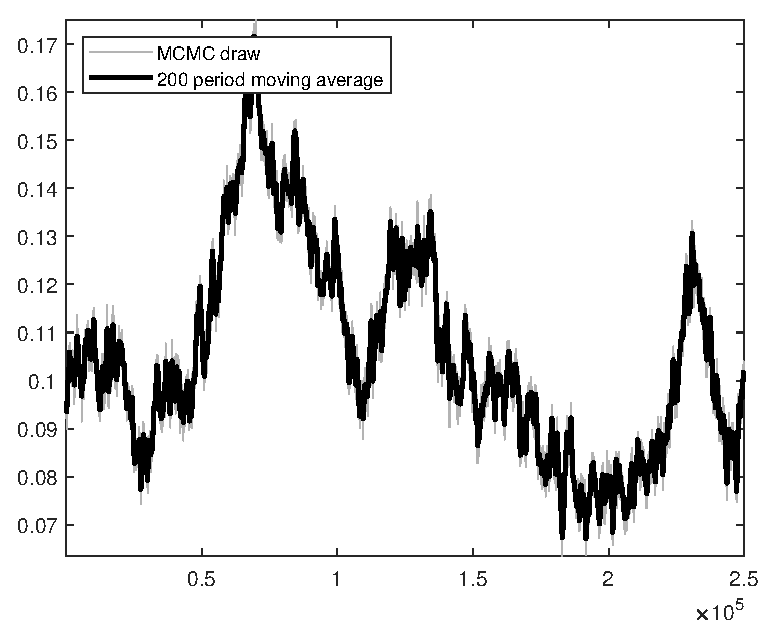
\includegraphics[width=0.8\textwidth]{SU_sectoral_perfect_mobility/graphs/TracePlot_eta_blck_1}\\
    \caption{Trace plot for parameter ${\eta}$ (block number 1).}
\end{figure}
 
\begin{figure}[H]
\centering
  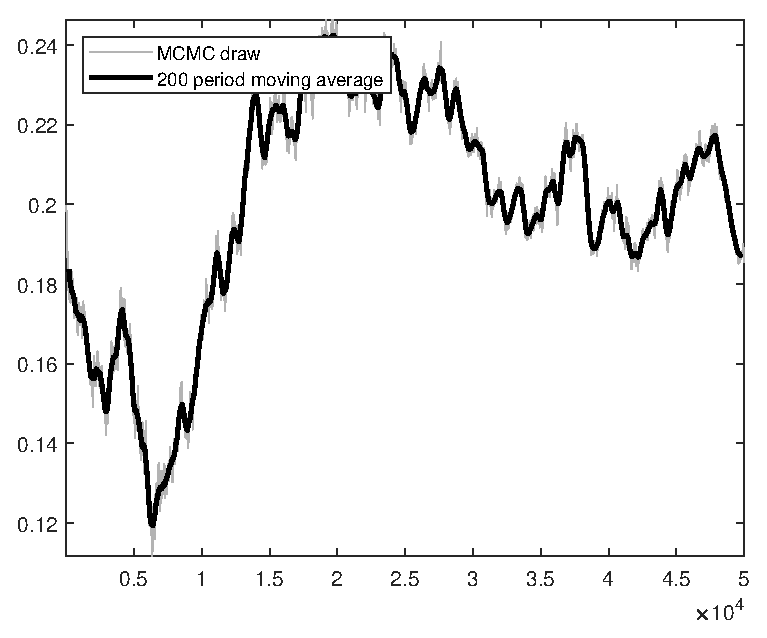
\includegraphics[width=0.8\textwidth]{SU_sectoral_perfect_mobility/graphs/TracePlot_nu_R_blck_1}\\
    \caption{Trace plot for parameter ${\nu_R}$ (block number 1).}
\end{figure}
 
\include{SU_sectoral_perfect_mobility/graphs/SU_sectoral_perfect_mobility_TracePlot_phi_blck_1} 
\end{document} 
